\documentclass[letterpaper]{article} % DO NOT CHANGE THIS
\usepackage[submission]{aaai2027}  % DO NOT CHANGE THIS
% The serif, sans-serif, and monospaced fonts are loaded automatically by
% aaai2027.sty (newtxtext, helvet, courier). DO NOT add \usepackage{times},
% \usepackage{helvet}, \usepackage{courier}, or any other font package.
\usepackage[hyphens]{url}  % DO NOT CHANGE THIS
\usepackage{graphicx} % DO NOT CHANGE THIS
\urlstyle{rm} % DO NOT CHANGE THIS
\def\UrlFont{\rm}  % DO NOT CHANGE THIS
\usepackage{natbib}  % DO NOT CHANGE THIS AND DO NOT ADD ANY OPTIONS TO IT
\usepackage{caption} % DO NOT CHANGE THIS AND DO NOT ADD ANY OPTIONS TO IT
\frenchspacing  % DO NOT CHANGE THIS
%
% These are recommended to typeset algorithms but not required. See the subsubsection on algorithms. Remove them if you don't have algorithms in your paper.
\usepackage{algorithm}
\usepackage{algorithmic}
\usepackage{amsfonts}

%
% These are recommended to typeset listings but not required. See the subsubsection on listing. Remove this block if you don't have listings in your paper.
\usepackage{newfloat}
\usepackage{listings}
\DeclareCaptionStyle{ruled}{labelfont=normalfont,labelsep=colon,strut=off} % DO NOT CHANGE THIS
\lstset{%
	basicstyle={\footnotesize\ttfamily},% footnotesize acceptable for monospace
	numbers=left,numberstyle=\footnotesize,xleftmargin=2em,% show line numbers, remove this entire line if you don't want the numbers.
	aboveskip=0pt,belowskip=0pt,%
	showstringspaces=false,tabsize=2,breaklines=true}
\floatstyle{ruled}
\newfloat{listing}{tb}{lst}{}
\floatname{listing}{Listing}

%
% Recommended for better-looking tables
\usepackage{booktabs}

%
% Keep the \pdfinfo as shown here. There's no need
% for you to add the /Title and /Author tags.
\pdfinfo{
/TemplateVersion (2027.1)
}

% DISALLOWED PACKAGES
% \usepackage{authblk} -- This package is specifically forbidden
% \usepackage{balance} -- This package is specifically forbidden
% \usepackage{CJK} -- This package is specifically forbidden
% \usepackage{float} -- This package is specifically forbidden
% \usepackage{flushend} -- This package is specifically forbidden
% \usepackage{fullpage} -- This package is specifically forbidden
% \usepackage{geometry} -- This package is specifically forbidden
% \usepackage{hyperref} -- This package is specifically forbidden
% \usepackage{navigator} -- This package is specifically forbidden
% (or any other package that embeds links such as navigator or hyperref)
% \usepackage{indentfirst} -- This package is specifically forbidden
% \usepackage{layout} -- This package is specifically forbidden
% \usepackage{multicol} -- This package is specifically forbidden
% \usepackage{nameref} -- This package is specifically forbidden
% \usepackage{savetrees} -- This package is specifically forbidden
% \usepackage{setspace} -- This package is specifically forbidden
% \usepackage{stfloats} -- This package is specifically forbidden
% \usepackage{tabu} -- This package is specifically forbidden
% \usepackage{titlesec} -- This package is specifically forbidden
% \usepackage{tocbibind} -- This package is specifically forbidden
% \usepackage{ulem} -- This package is specifically forbidden
% \usepackage{wrapfig} -- This package is specifically forbidden
% DISALLOWED COMMANDS
% \nocopyright -- Your paper will not be published if you use this command
% \addtolength -- This command may not be used
% \balance -- This command may not be used
% \baselinestretch -- Your paper will not be published if you use this command
% \clearpage -- No page breaks of any kind may be used for the final version of your paper
% \columnsep -- This command may not be used
% \newpage -- No page breaks of any kind may be used for the final version of your paper
% \pagebreak -- No page breaks of any kind may be used for the final version of your paper
% \pagestyle -- This command may not be used
% \tiny -- This is not an acceptable font size.
% \vspace{- -- No negative value may be used in proximity of a caption, figure, table, section, subsection, subsubsection, or reference
% \vskip{- -- No negative value may be used to alter spacing above or below a caption, figure, table, section, subsection, subsubsection, or reference

\setcounter{secnumdepth}{0} %May be changed to 1 or 2 if section numbers are desired.

% The file aaai2027.sty is the style file for AAAI Press
% proceedings, working notes, and technical reports.
%

% Title

% Your title must be in mixed case, not sentence case.
% That means all verbs (including short verbs like be, is, using,and go),
% nouns, adverbs, adjectives should be capitalized, including both words in hyphenated terms, while
% articles, conjunctions, and prepositions are lower case unless they
% directly follow a colon or long dash
\title{Dual-Expert Keys for Reducing False-Positive Retrieval in Lifelong Vision–Language Model Editing}
\author{
    %Authors
    % All authors must be in the same font size and format.
    Written by AAAI Press Staff\textsuperscript{\rm 1}\thanks{With help from the AAAI Publications Committee.}\\
    AAAI Style Contributions by Peter Patel Schneider,
    Sunil Issar,\\
    J. Scott Penberthy,
    George Ferguson,
    Hans Guesgen,
    Francisco Cruz\equalcontrib\corresponding,
    Marc Pujol-Gonzalez\equalcontrib\corresponding
}
\affiliations{
    %Afiliations
    \textsuperscript{\rm 1}Association for the Advancement of Artificial Intelligence\\
    % If you have multiple authors and multiple affiliations
    % use superscripts in text and roman font to identify them.
    % For example,

    % Sunil Issar\textsuperscript{\rm 2},
    % J. Scott Penberthy\textsuperscript{\rm 3},
    % George Ferguson\textsuperscript{\rm 4}\corresponding,
    % Hans Guesgen\textsuperscript{\rm 5}
    % Note that the comma should be placed after the superscript

    1101 Pennsylvania Ave, NW Suite 300\\
    Washington, DC 20004 USA\\
    % email address must be in roman text type, not monospace or sans serif
    proceedings-questions@aaai.org
%
% See more examples next
}

%Example, Single Author, ->> remove \iffalse,\fi and place them surrounding AAAI title to use it
\iffalse
\title{My Publication Title --- Single Author}
\author {
    Author Name
}
\affiliations{
    Affiliation\\
    Affiliation Line 2\\
    name@example.com
}
\fi

\iffalse
%Example, Multiple Authors, ->> remove \iffalse,\fi and place them surrounding AAAI title to use it
\title{My Publication Title --- Multiple Authors}
\author {
    % Authors
    First Author Name\textsuperscript{\rm 1,\rm 2}\equalcontrib,
    Second Author Name\textsuperscript{\rm 2}\equalcontrib,
    Third Author Name\textsuperscript{\rm 1}\corresponding
}
\affiliations {
    % Affiliations
    \textsuperscript{\rm 1}Affiliation 1\\
    \textsuperscript{\rm 2}Affiliation 2\\
    firstAuthor@affiliation1.com, secondAuthor@affilation2.com, thirdAuthor@affiliation1.com
}
\fi


\begin{document}

\maketitle

% \begin{abstract}
% Lifelong vision--language editors can look correct on the image they were edited for, then still emit the new fact when the scene is only visually related. In our probes this is usually not soft overwrite of the base model. It is false-positive retrieval  (false-cross): weak visual keys make a different stored edit look good enough to retrieve, so the wrong expert fires.
% We address it in two steps. Dual-Expert Keys let an edit fire only when the visual match and the prompt-key match both pass. Separately, adversarial visual binding training attaches each edit to its correct image and lowers expert activation when the image is swapped or a hard negative. On VLKEB-based adversarial grounding probes, Dual-Expert Keys cut swap false-positive retrieval rate from 96\% to 46\% over five seeds and keep reliability near 94\%. Adversarial visual binding training complements Dual-Expert Keys by stabilizing edit–image binding under these adversarial probes. Against Fine-tuning, MEND-VL, and SERAC-VL on the same probes, we keep high reliability while directly reducing the wrong-expert retrieval rate.
% \end{abstract}

\begin{abstract}
    Lifelong vision–language model editors store sequential edits in a growing expert pool and retrieve relevant experts at inference time. Although these systems can achieve high reliability on edited examples, routing logs reveal a distinct grounding failure: when the prompt is held fixed but the image is swapped or replaced by a hard negative, the editor frequently activates an expert associated with a different scene. Standard reliability, generality, and locality metrics do not expose this behavior. We formalize it as false-positive retrieval and evaluate it using adversarial grounding probes constructed from VLKEB and EVQA. To reduce this failure, we introduce Dual-Expert Keys (DEK), which allow an expert to activate only when it passes both a prototype-relative visual gate and a prompt-key gate. We further introduce adversarial visual binding training (AVBT), which strengthens edit–image association by suppressing expert activation on mismatched images. On a BLIP-2 OPT-2.7B lifelong mixture-of-experts editor, DEK reduces VLKEB image-swap false-positive retrieval from 96\% to 46\% across five evaluation seeds while preserving 93.7\% reliability and maintaining standard generality and locality. Additionally, on a cross-dataset setup on EVQA using hard-negative images, false-positive retrieval fall from 96.8\% to 2.7\%, with reliability remaining near 95\%. These results identify retrieval leakage as a distinct failure mode in lifelong multimodal editing and demonstrate that dual-modal gating can substantially improve retrieval safety without sacrificing edit reliability.
\end{abstract}

% Uncomment the following to link to your code, datasets, an extended version or similar.
% You must keep this block between (not within) the abstract and the main body of the paper.
% Make sure that you do not de-anonymize yourself with these links.
% \begin{links}
%     \link{Code}{https://aaai.org/example/code}
%     \link{Datasets}{https://aaai.org/example/datasets}
%     \link{Extended version}{https://aaai.org/example/extended-version}
% \end{links}

\section{Introduction}
% Large vision--language models (VLMs) now answer questions about photographs, documents, and everyday scenes, and they are often treated as soft knowledge bases in interactive systems~\cite{li2023blip2}.
% Facts encoded in these models drift: places change names, entities are mislabeled, and new visual knowledge appears after pre-training ends.
% Full fine-tuning is costly and can disturb unrelated skills, so \emph{model editing} has emerged as a practical alternative apply a local update that corrects a target fact while preserving behaviour elsewhere~\cite{Mitchell2021FastME,mitchell2022serac,cheng2023mmedit}.
% Multimodal benchmarks such as MMEdit and VLKEB standardize this goal around reliability, generality, and locality~\citep{cheng2023mmedit,huang2024vlkeb}.
% When edits must arrive one after another, the problem becomes \emph{lifelong} editing: each new fact joins a growing set of updates that must remain available without overwriting earlier ones~\citep{chen2025liveedit}.

Large vision-language models (VLMs) can answer questions about photographs, documents, and everyday scenes, and increasingly serve as implicit knowledge bases in interactive systems~\citep{li2023blip2}. However, the knowledge encoded in these models may become outdated or inaccurate as entities change, annotations are corrected, and new visual information emerges after pretraining. Updating the entire model through fine-tuning is computationally expensive and may degrade orthogonal capabilities. Model editing therefore provides an attractive alternative by introducing targeted corrections while preserving model behaviour on unrelated inputs~\citep{Mitchell2021FastME,mitchell2022serac,cheng2023mmedit}. Multimodal editing benchmarks such as MMEdit and VLKEB evaluate this objective through reliability, generality, and locality~\citep{cheng2023mmedit,huang2024vlkeb}. In lifelong editing, the challenge is further complicated by a sequence of updates that must coexist without overwriting previously acquired knowledge~\citep{chen2025liveedit}.

% Retrieval- and mixture-of-experts (MoE) editors are a natural fit for that setting.
% They store each edit as an expert (or memory entry) and, at test time, retrieve which expert(s) to inject for a query~\citep{mitchell2022serac,chen2025liveedit}.
% On the image used for the edit, these systems can look excellent: reliability often sits in the low-to-mid 90s.
% The harder question is whether the edit is \emph{visually grounded}.
% Consider a city-entity edit with prompt $p$ (``What city in Illinois is depicted in the image?'') and target answer ``Kankakee.''
% With the edited photograph, the post-edit model answers correctly.
% With the \emph{same} prompt but a swapped skyline or a confusable hard-negative scene, a retrieval editor can still surface ``Kankakee'' (Figure~\ref{fig:teaser}).
% That behaviour is especially damaging in lifelong pools: the more experts accumulate, the more chances a weak visual key has to match the wrong past edit.

Retrieval-based and mixture-of-experts editors are well suited to lifelong editing because they can store each update as an expert or memory entry while leaving the backbone model unchanged~\citep{mitchell2022serac,chen2025liveedit}. At inference time, the editor retrieves the experts considered relevant to the current query and injects their corresponding residual updates. Although these systems can achieve high reliability on the images used during editing, high reliability does not necessarily imply that the edited knowledge is visually grounded. For example, consider an edit that associates a photograph with the answer ``Kankakee'' (Figure~\ref{fig:teaser}) for the question ``What city in Illinois is depicted in the image?'' The edited model may answer correctly when presented with the original photograph, yet continue to produce the same answer when the photograph is replaced by an unrelated skyline or a visually confusable scene. This problem becomes increasingly consequential as the expert pool grows because additional stored edits create more opportunities for an unrelated expert to be selected.


% We find that this failure is usually not soft overwrite of the frozen base VLM.
% On our adversarial grounding probes, routing logs show that a \emph{foreign} stored expert is retrieved for the swapped image often at rates above 90\%.
% We call this \emph{false-positive retrieval} (and \emph{false-cross} when we score it from expert identities): the visual key for edit $i$ is similar enough to query image $j\neq i$ that the wrong expert passes the retrieval threshold and injects the wrong fact.
% This is a retrieval-safety problem, not merely an answer-quality problem. Yet the metrics that dominate multimodal editing papers reliability on the edited image, text/image generality, and locality on unrelated prompts~\citep{cheng2023mmedit,huang2024vlkeb,chen2025liveedit} do not report which expert fired under image-swap or hard-negative probes.

Our analysis indicates that this behaviour is frequently caused by incorrect expert selection rather than interference with the parameters of the frozen VLM. On the proposed adversarial grounding probes, routing logs show that experts associated with other images are often activated at rates exceeding 90\%. We refer to this failure as \emph{false-positive retrieval}. It occurs when an unrelated stored expert receives a sufficiently high retrieval score to pass the routing threshold and inject an incorrect fact. False-positive retrieval is therefore a routing safety failure that is distinct from answer-level accuracy. Standard evaluations based on reliability, generality, and locality do not reveal which expert is activated when the prompt is preserved but the image is replaced by a mismatched or confusable alternative~\citep{cheng2023mmedit,huang2024vlkeb,chen2025liveedit}.


% \begin{figure*}[t]
% \centering
% 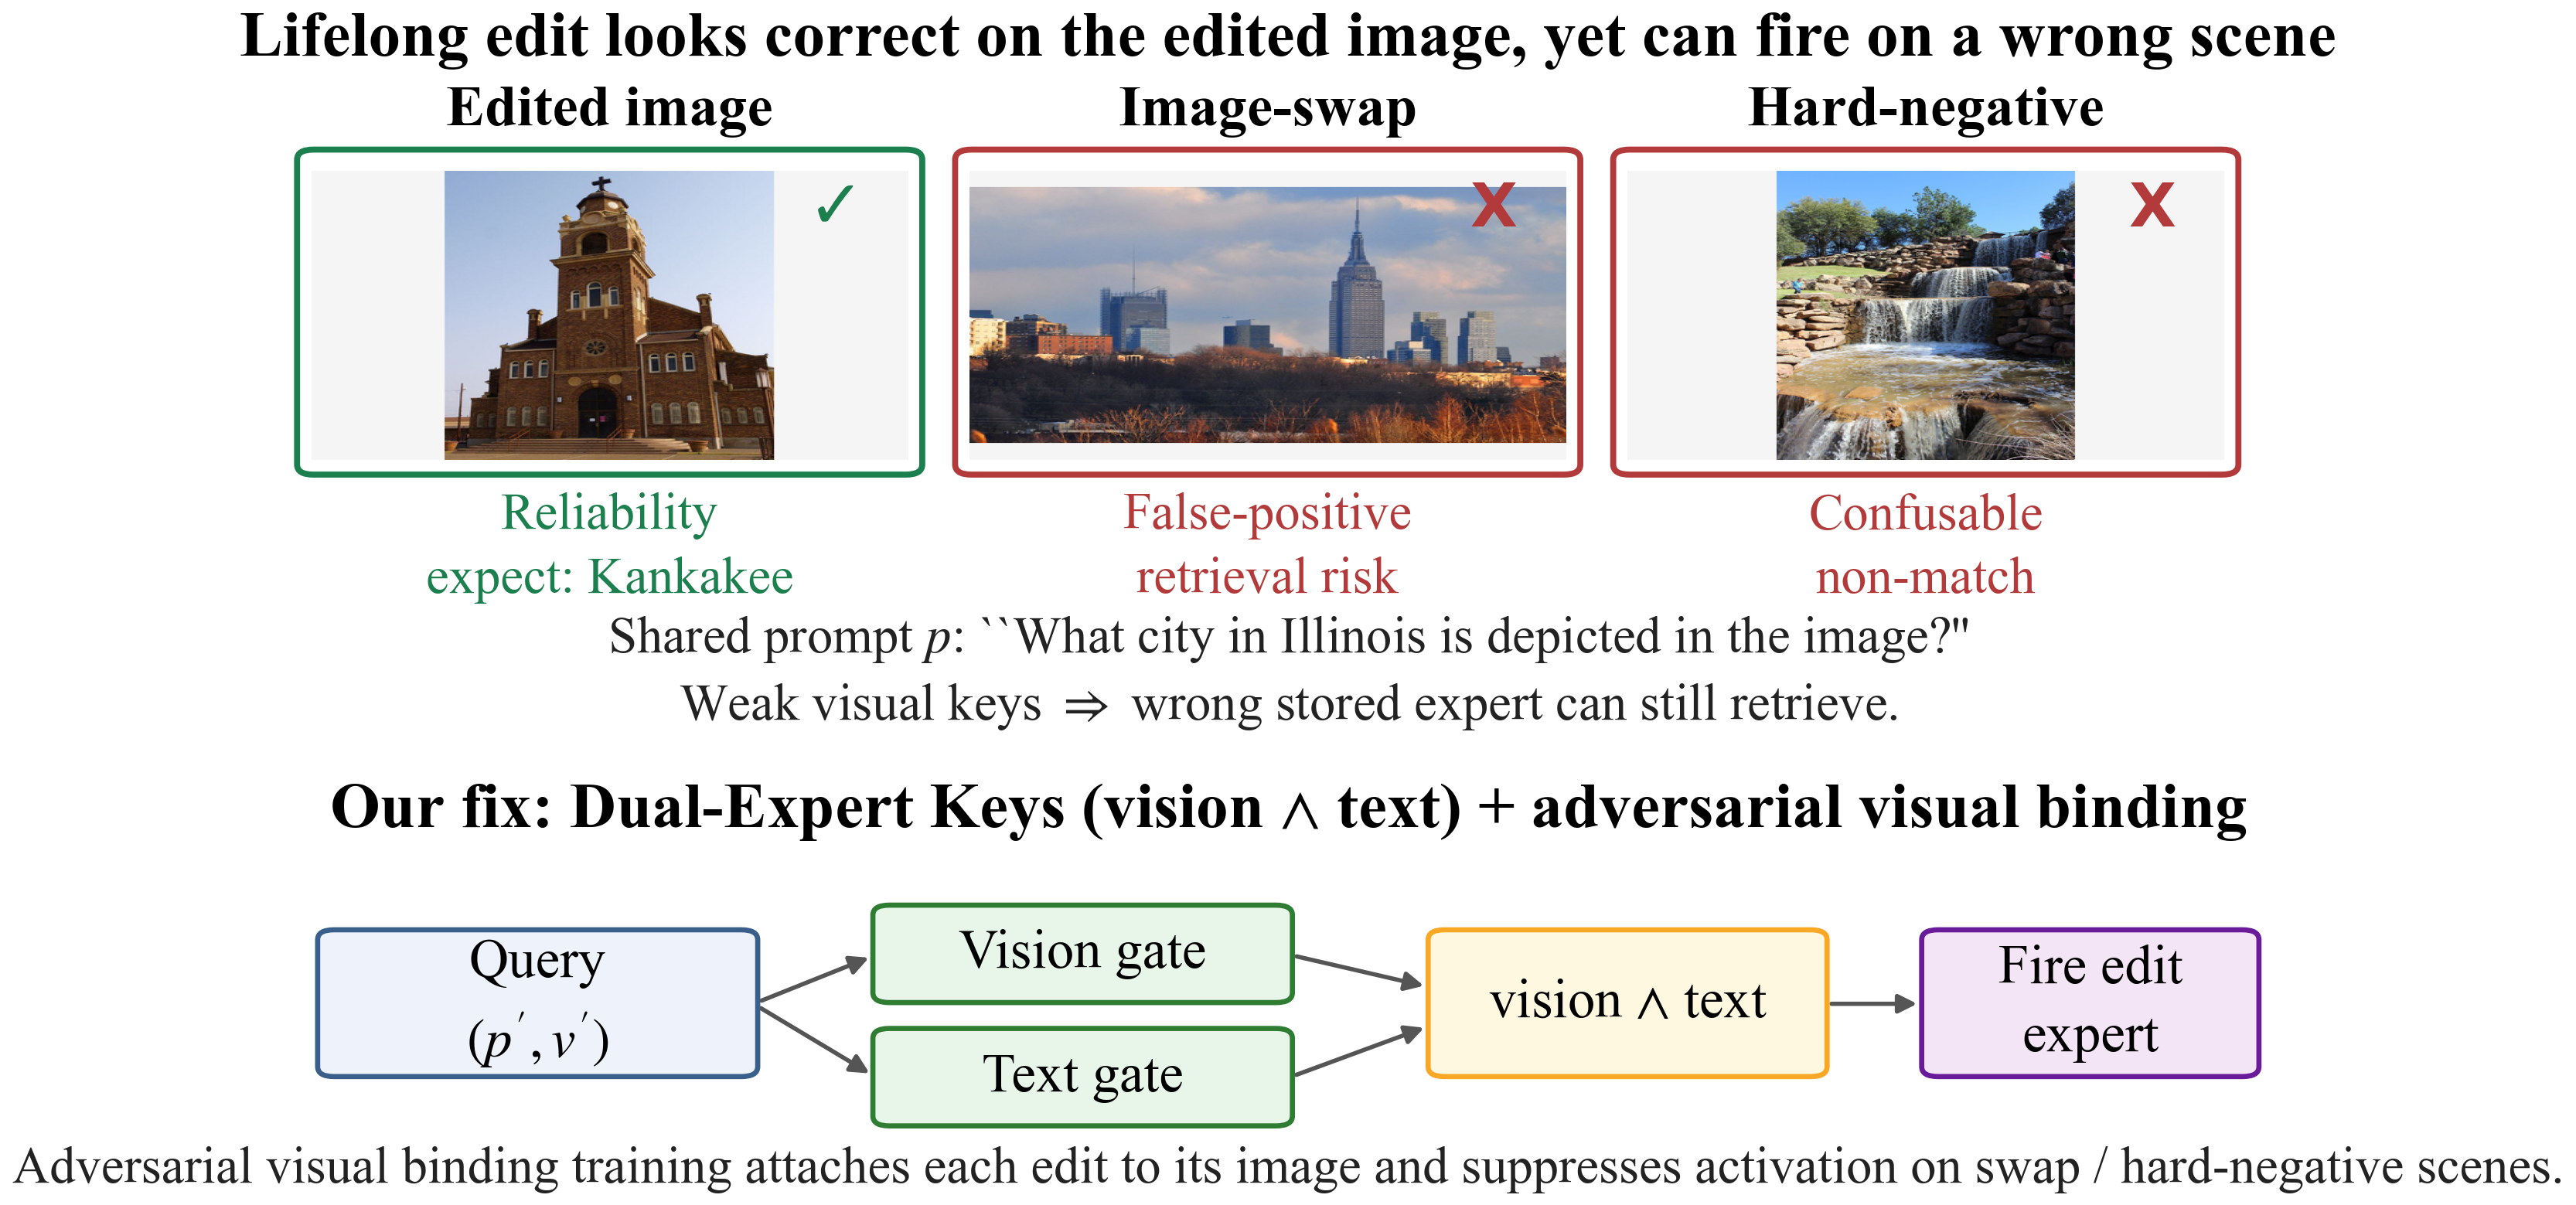
\includegraphics[height=0.16\textheight,keepaspectratio]{Figures/fig1_teaser_v5.png}
% \caption{Top: shared prompt with the edited image (reliability), an image-swap, and a hard-negative.
% Bottom: Dual-Expert Keys fire an edit only when vision and text gates both pass; adversarial visual binding strengthens edit-image attachment under these probes.}
% \label{fig:teaser}
% \end{figure*}
\begin{figure}[t]
\centering
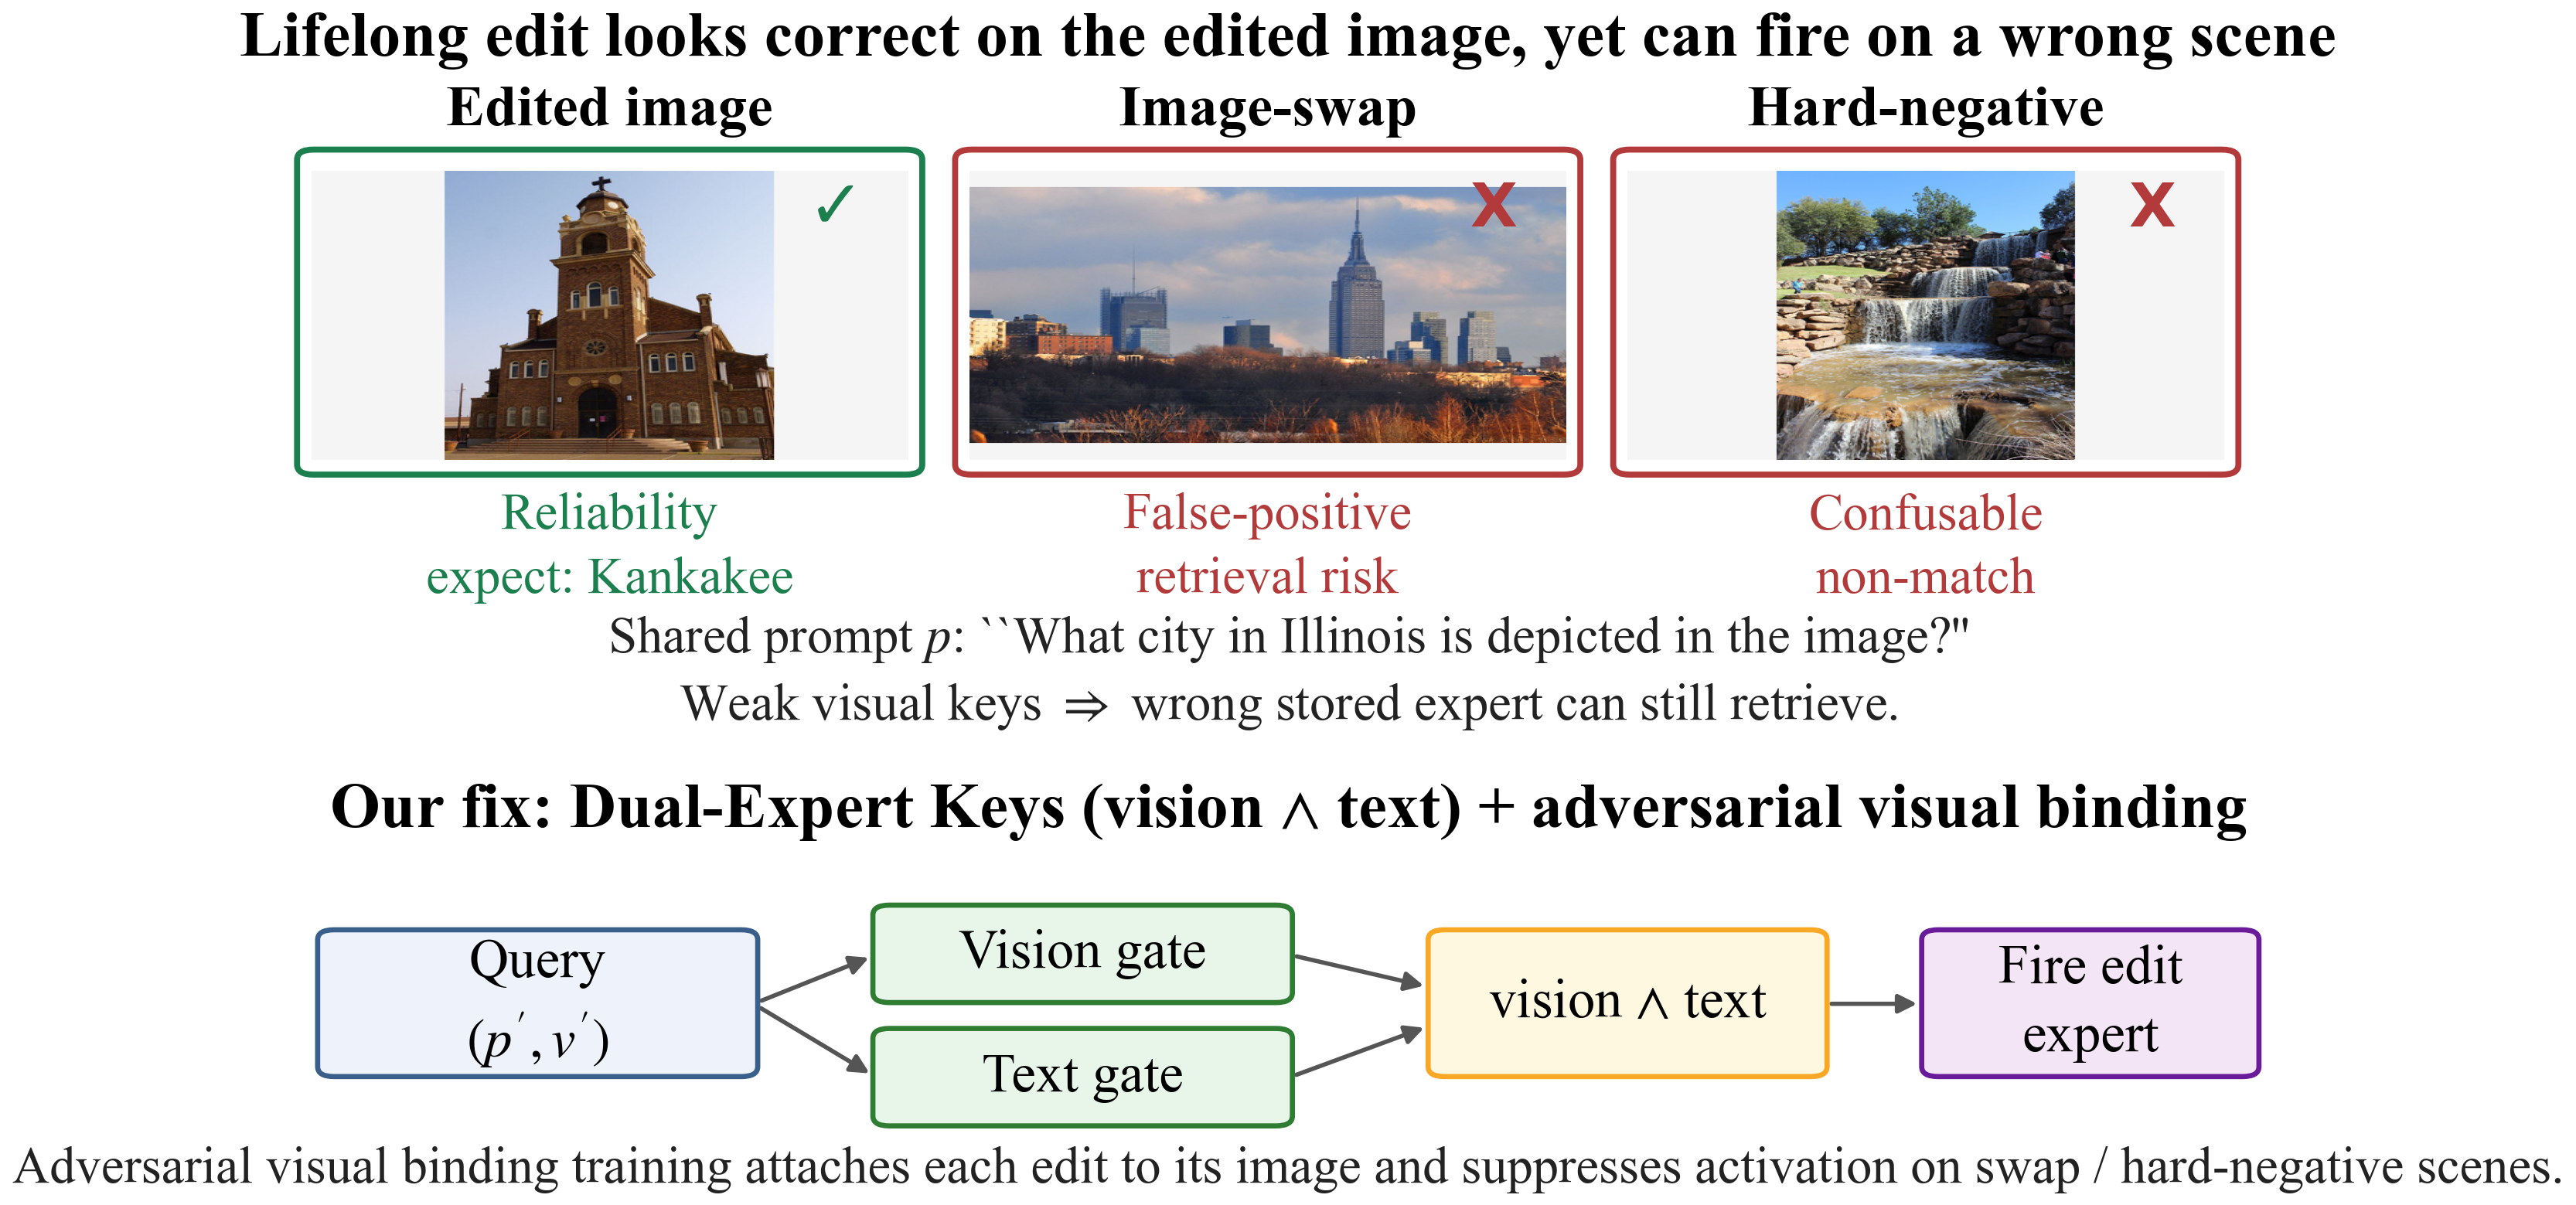
\includegraphics[width=\columnwidth]{Figures/fig1_teaser_v5.png}
\caption{Top: shared prompt with the edited image (reliability), an image-swap, and a hard-negative.
Bottom: Dual-Expert Keys fire an edit only when vision and text gates both pass; adversarial visual binding strengthens edit--image attachment under these probes.}
\label{fig:teaser}
\end{figure}

% Lifelong VLM editors such as LiveEdit already combine visual filtering with text routing~\citep{chen2025liveedit}, but those designs are optimized for Rel/Gen/Loc, not for measuring or blocking wrong-expert activation on adversarial images.
% DualEdit studies \emph{where} to place modality-specific adapters for reliability--locality trade-offs~\citep{shi2025dualedit}; it does not address lifelong expert-pool leakage.
% Weight-updating editors (Fine-tuning, MEND, SERAC)~\citep{Mitchell2021FastME,mitchell2022serac} can rewrite answers, but when the competing system is a growing expert memory they leave false-positive retrieval unmeasured.

Existing multimodal editors do not directly address this failure. LiveEdit combines visual filtering with textual routing, but its retrieval mechanism and evaluation are designed primarily around reliability, generality, and locality rather than the activation of unrelated experts under adversarial images~\citep{chen2025liveedit}. DualEdit investigates the placement of modality-specific adapters and the resulting trade-off between reliability and locality, rather than retrieval leakage in a growing expert pool~\citep{shi2025dualedit}. Other editing approaches, including Fine-tuning, MEND-VL, and SERAC-VL, provide relevant comparisons for answer-level editing performance but do not expose the same growing set of expert identities required to measure false-positive retrieval directly~\citep{Mitchell2021FastME,mitchell2022serac,cheng2023mmedit}. Consequently, a system may perform well under standard editing metrics while still activating an unrelated stored edit when the visual context changes.

% \paragraph{Key insight.}
% If leakage is dominated by wrong-expert selection, then improving only the binding of an edit to its own image is not enough: the retrieval rule itself must reject candidates unless \emph{both} modalities agree.
% A vision-only gate can still admit a foreign edit whose visual key collides with the query; a text-only gate can still admit that edit when the prompt matches.
% Requiring vision $\wedge$ text agreement turns retrieval into a dual check: the image must look like the edited scene \emph{and} the prompt must match the stored edit key.

Addressing this problem requires modifying both expert retrieval and the association between an edit and its source image. Strengthening only the visual binding of an expert is insufficient when unrelated experts can still pass the retrieval threshold. Similarly, routing based on either visual or textual evidence alone can admit incorrect experts. A visual gate may accept an expert with a colliding image representation, whereas a textual gate may accept an expert because multiple edits share similar prompts. We therefore require agreement between the visual evidence and the prompt before an expert can be activated.

% \paragraph{Our approach.}
% We study this failure on a lifelong MoE-style editor~\citep{chen2025liveedit} with BLIP-2~\citep{li2023blip2} as the frozen backbone the setting where continuous expert pools make false-positive retrieval observable.
% We introduce two complementary pieces.
% (1)~\emph{Dual-Expert Keys (DEK)}: at inference, an expert may fire only when its visual gate and its prompt-key (text) gate both pass.
% (2)~\emph{Adversarial visual binding training (AVBT)}: during editing, we attach each expert to its correct image and explicitly suppress fused expert activation on swap and hard-negative images.
% DEK is the primary anti-leakage mechanism; AVBT stabilizes edit--image binding so the dual-gate is not fighting a weakly grounded expert.

Based on this principle, we introduce DEK, a retrieval mechanism that maintains separate visual and textual keys for each stored edit. At inference time, an expert is activated only when it satisfies both a prototype-relative visual gate and a prompt-key gate. We complement this mechanism with AVBT, which encourages activation on the correct edited image while suppressing expert activation on image swaps and hard negatives. DEK directly changes the routing decision, whereas AVBT strengthens the visual association on which the routing mechanism operates. We instantiate both components within a lifelong mixture-of-experts editor using BLIP-2 as the frozen VLM backbone~\citep{li2023blip2,chen2025liveedit}.

% \paragraph{Empirical preview.}
% On VLKEB-based adversarial grounding probes~\citep{huang2024vlkeb}, Dual-Expert Keys cut the swap false-positive retrieval rate from $96\%$ to $46\%$ over five evaluation seeds while keeping reliability near $94\%$.
% Standard Rel/Gen/Loc stay essentially on parity with the lifelong baseline.
% Ablations show that binding training alone leaves false-positive retrieval near $96\%$; adding Dual-Expert Keys is what halves wrong-expert retrieval.
% Under a matched long-form train/eval protocol, false-positive retrieval similarly falls from $88\%$ to $38\%$ with reliability held near $73\%$.
% Against Fine-tuning, MEND-VL, and SERAC-VL on the same probes, our method is the one that keeps high reliability while directly reducing wrong-expert retrieval.
% We emphasize the claim carefully: we target \emph{anti-leakage routing}, not token-level image-swap state of the art.

Experiments on adversarial grounding probes constructed from VLKEB demonstrate that DEK reduces the image-swap false-positive retrieval rate from $96\%$ to $46\%$ across five evaluation seeds while preserving $94\%$ reliability. Reliability, textual generality, multimodal generality, and locality remain comparable to those of the lifelong baseline. Component ablations show that adversarial binding alone leaves the false-positive retrieval rate near $96\%$, indicating that the dual-expert retrieval mechanism is responsible for the substantial reduction in incorrect expert activation. 
% Under a matched long-form training and evaluation protocol, DEK similarly reduces false-positive retrieval from $88\%$ to $38\%$ while maintaining reliability near $73\%$. 
The same pattern generalizes to EVQA, where DEK reduces hard-negative false-positive retrieval from $96.8\%$ to $2.7\%$ while preserving reliability near $95\%$. Comparisons with Fine-tuning, MEND-VL, and SERAC-VL on the same adversarial probes further show that DEK uniquely maintains high reliability while directly reducing incorrect expert retrieval. Our objective is to prevent retrieval leakage rather than to achieve state-of-the-art token-level accuracy under image swaps.


% \paragraph{Contributions.}
% This paper makes three contributions:
% \begin{itemize}
%     \item \textbf{Problem.} We characterize false-positive retrieval (false-cross) as a dominant visual grounding failure in lifelong multimodal editors under image-swap and hard-negative probes, and show that it is under-reported by Rel/Gen/Loc alone.
%     \item \textbf{Method.} We propose Dual-Expert Keys, which require vision--text agreement at retrieval time, together with adversarial visual binding training that attaches edits to their images and suppresses adversarial activation.
%     \item \textbf{Evidence.} On VLKEB grounding probes we show large false-positive cuts with reliability preserved, ablations that isolate Dual-Expert Keys as the false-positive retrieval mechanism, multi-seed stability, and comparisons to Fine-tuning, MEND-VL, and SERAC-VL.
% \end{itemize}

% The rest of the paper covers Related Work, Problem, Method, Experiments, Results, Limitations, and Conclusion.

The main contributions of this work are as follows:
\begin{itemize}
    \item We identify and formalize false-positive retrieval as a visual grounding failure in lifelong multimodal editing. We introduce image-swap and hard-negative probes that expose incorrect expert activation not captured by standard reliability, generality, and locality metrics.
    
    \item We propose Dual-Expert Keys, which require agreement between visual and textual retrieval signals before an expert can be activated. We further introduce adversarial visual binding training to strengthen the association between each edit and its corresponding image.
    
    \item We demonstrate substantial and stable reductions in false-positive retrieval in both within-benchmark on VLKEB and cross-dataset setup on EVQA. On both datasets, DEK reduces false-positive retrieval while preserving high reliability and standard editing performance.
\end{itemize}

\section{Related Work}
\label{sec:related}

\paragraph{Knowledge editing for language models.}
Modern language models store large amounts of factual knowledge, but that knowledge can be wrong, outdated, or incomplete.
Model editing aims to inject a local correction without full retraining and without broadly damaging unrelated behaviour~\citep{decao2021knowledgeeditor,yao2023editing}.
The literature is usually grouped into three families.
Locate-then-edit methods first identify parameters associated with a fact and then rewrite them; ROME does this for single edits, and MEMIT scales the idea to many facts~\citep{meng2022rome,meng2023memit}.
Meta-learning editors such as MEND train a hypernetwork to turn edit gradients into low-rank weight updates~\citep{Mitchell2021FastME}.
Memory-based retrieval editors keep the base model frozen and store edits externally. SERAC retrieves a counterfactual memory and routes through a scope classifier~\citep{mitchell2022serac}, GRACE maintains lifelong discrete key-value adaptors~\citep{hartvigsen2023grace}, and in-context editors such as IKE place edit demonstrations in the prompt~\citep{zheng2023ike}.
EasyEdit unifies many of these methods behind a common interface, which has made fair comparison easier~\citep{wang2024easyedit}.
Beyond single-fact reliability, later evaluation work asks whether an edit propagates consistently to related facts~\citep{cohen2024evaluating} and whether editors can handle long or diverse-format targets~\citep{jiang2025anyedit}.
AnyEdit extends long-form text editing; it decomposes targets into chunks and updates them autoregressively, one segment at a time rather than a single pass~\citep{jiang2025anyedit}.

\paragraph{Multimodal knowledge editing and benchmarks.}
Editing vision-language models is harder than editing text-only language models because the fact is tied to an image as well as a prompt~\citep{cheng2023mmedit}.
MMEdit established early multimodal reliability, generality, and locality protocols for VQA- and caption-style edits~\citep{cheng2023mmedit}.
VLKEB improves visual quality by building edits from multimodal knowledge graphs and adds portability-oriented checks~\citep{huang2024vlkeb}.
More recent benchmarks push different axes. MC-MKE emphasizes modality consistency across fine-grained edit formats~\citep{zhang2025mcmke}, MMKE-Bench covers diverse visual semantics and free-form knowledge~\citep{jiang2025mmke}, and ComprehendEdit aggregates multiple tasks with generalization and preservation indices~\citep{ma2025comprehendedit}.
On the method side, DualEdit studies where to edit. It updates text and vision at modality-sensitive layers and uses a gate to protect original behaviour~\citep{shi2025dualedit}.
That gating is about reliability-locality trade-offs under layer choice, not about blocking wrong-expert retrieval in a lifelong MoE pool.
Across this literature, success is still mostly reported as whether the new answer appears on the edited (or rephrased) input, and unrelated inputs stay stable.
What is usually missing is an explicit account of which stored edit fired when the prompt is held fixed and the image is swapped or made confusable.

\paragraph{Lifelong retrieval editors and visual keys.}
Lifelong editing requires many updates to coexist over time~\citep{hartvigsen2023grace,chen2025liveedit}.
LiveEdit is the closest system to our setting. It generates a low-rank MoE expert per edit, stores experts in a growing repository, and at inference uses hard visual filtering followed by soft text routing to fuse relevant experts into a frozen VLM such as BLIP-2~\citep{chen2025liveedit,li2023blip2}.
Related multimodal backbones used in editing studies include LLaVA and InstructBLIP~\citep{liu2023llava,dai2023instructblip}.
Because retrieval decides which residual is injected, routing quality becomes part of editing safety as the pool grows an issue that sparse MoE selection has long faced in other domains~\citep{shazeer2017moe}.
Strong visual encoders can help in principle. CLIP-style vision-language similarity~\citep{radford2021clip} and DINOv2 features~\citep{oquab2024dinov2} often separate images well in offline probes.
But offline discrimination does not automatically transfer to edit retrieval when the editor compresses vision into a few routing keys and scores them against a large lifelong pool.
Weight-updating multimodal adaptations of Fine-tuning, MEND, and SERAC remain important baselines~\citep{Mitchell2021FastME,mitchell2022serac,cheng2023mmedit}; they can change answers, yet they do not expose a growing expert identity that we can score for false-cross.

% \paragraph{Positioning and distinction from close neighbours.}
% Our focus is an under-measured lifelong multimodal failure: \emph{false-positive retrieval} (false-cross) under image-swap and hard-negative probes.
% Dual-Expert Keys require vision $\wedge$ text agreement before an expert may fire; adversarial visual binding training attaches each edit to its image and suppresses activation on adversarial scenes.
% This differs from DualEdit, which chooses modality-specific layers and a Rel/Loc gate~\citep{shi2025dualedit}.
% It also differs from benchmark papers that expand Rel/Gen/Loc, portability, or modality consistency without measuring wrong-expert retrieval rates~\citep{huang2024vlkeb,zhang2025mcmke,jiang2025mmke,ma2025comprehendedit}.
% We use a LiveEdit-style lifelong MoE editor as the experimental \emph{testbed} because continuous expert pools make false-cross observable and actionable.
% The scientific claim is not ``higher Rel/Gen/Loc than LiveEdit on the original leaderboard,'' but a diagnosis and mechanism for anti-leakage retrieval under adversarial images.

Taken together, prior editing methods and multimodal benchmarks have made reliability, generality, and locality the default success criteria~\citep{cheng2023mmedit,huang2024vlkeb,chen2025liveedit}.
Those criteria ask whether the edited answer appears on the intended or rephrased input, and whether unrelated inputs remain stable.
They do not ask, under a shared prompt and an adversarial image, whether a lifelong pool retrieves a foreign expert.
As a result, false-positive retrieval under image-swap and hard-negative conditions remains largely unmeasured, even in settings where continuous expert pools make that failure observable.


\section{Problem Defination}
\label{sec:problem}

Lifelong multimodal editors that store one expert per edit are attractive precisely because the base VLM can stay frozen.
As edits accumulate, however, the system is only as safe as its retrieval step.
Write $\mathcal{E}=\{e_1,\ldots,e_m\}$ for the current expert pool, and let each $e_i$ remember an edit $(p_i,x_i,y_i)$ a prompt, an image, and a target answer.
Given a new query $(p,x)$, the editor scores the pool and injects one or more residuals into the frozen model.
On the photograph that was actually edited, this design can look excellent: reliability, generality, and locality numbers in the literature are often already high~\cite{cheng2023mmedit,huang2024vlkeb,chen2025liveedit}.
The awkward case is the one those scores largely ignore.
Keep the prompt fixed, replace the image with something else, and ask: does the pool still hand you an expert that belongs to a different scene?

To make that question concrete we use a small suite of \emph{adversarial grounding} probes built around the same edit prompt $p_i$ whenever we can.
Reliability puts the edited image $x_i$ back in front of the model; it answers the usual question of whether the edit took.
\emph{Image-swap} instead feeds another edit's image $x_j$ ($j\neq i$), so the text still asks for $y_i$ while the pixels show a different entity or place.
\emph{Hard-negative} keeps $p_i$ but substitutes a near-neighbour distractor that was never itself an edit image.
Text rephrases and ordinary locality checks stay in the protocol as controls.
If a text rephrase roughly tracks reliability, yet swap and hard-negative collapse, the trouble is unlikely to be ``the language model simply ignored the picture.''
Along the way we record not only token overlap with $y_i$, but also which pool experts actually fired routing identities and how many were retrieved.

That logging lets us separate two notions that are easy to conflate.
Answer-level swap or hard-negative accuracy tells you what the model said.
We care at least as much about which memory was opened.
We call it \emph{false-positive retrieval} when, for an adversarial query aimed at edit $i$, retrieval activates at least one expert $e_k$ with $k\neq i$.
The rate of that event is our main leakage number (lower is better).
In tables we write it \textbf{FPR}.
FPR is deliberately a retrieval-safety metric.
A non-zero token score on a wrong image can happen for many reasons, including ordinary generation from the frozen backbone.
A high FPR, by contrast, points at the lifelong pool: the editor selected a foreign expert and injected the corresponding fact.

Standard Rel, Gen and Loc reporting does not catch this.
Those metrics never ask, under a shared prompt and an adversarial image, whether the retrieved expert identity matches the scene on screen.
So a system can post strong on these while still admitting colliding visual keys as the pool grows.
Figure~\ref{fig:teaser} is the picture we have in mind: one prompt, three images (edited, swapped, hard-negative), and later a dual vision-text check before an expert is allowed to fire.

The empirical picture on our BLIP-2 lifelong MoE testbed~\cite{li2023blip2,chen2025liveedit} with VLKEB-derived probes~\cite{huang2024vlkeb} is hard to dismiss as a soft-overwrite story alone.
On the VLKEB evaluation split with our adversarial probes, reliability for the lifelong baseline sits near $94\%$, yet swap FPR climbs to $96\%$: the edit looks solid on its own photograph and still almost always retrieves someone else's expert under image-swap.
More broadly we see the same shape again and again strong own-image reliability, a wide gap once the image is swapped or made confusable, and FPR often above $90\%$ when many experts share a scalar visual key.
Results will show that teaching the editor to bind more tightly to its own image is not enough by itself.
If foreign experts keep clearing the retrieval bar, the decision rule has to change: an edit should fire only when the image evidence and the prompt key both agree.
That is the motivation for Dual-Expert Keys at inference and for adversarial visual binding during training.


\section{Methodology}
\label{sec:method}

We target false-positive retrieval directly with two coupled mechanisms (Figure~\ref{fig:arch}).
\emph{Dual-Expert Keys} change the inference rule: a stored edit may fire only when its vision evidence and its prompt-key evidence both agree with the query.
\emph{Adversarial visual binding} is the training counterpart: each edit is attached to its correct image and suppressed on swap and hard-negative images, so the dual gate is not fighting weakly grounded keys.
The two play different roles empirically binding improves adversarial answer behaviour somewhat, while Dual-Expert Keys are what cut false-positive retrieval roughly in half.
We instantiate the method on a frozen VLM with a growing pool of low-rank residuals, because that setting makes wrong-expert retrieval observable.
% ; the scientific claim is the retrieval-safety mechanism, not a new Rel/Gen/Loc leaderboard entry for any prior lifelong editor~\cite{chen2025liveedit}.


\begin{figure*}[t]
\centering
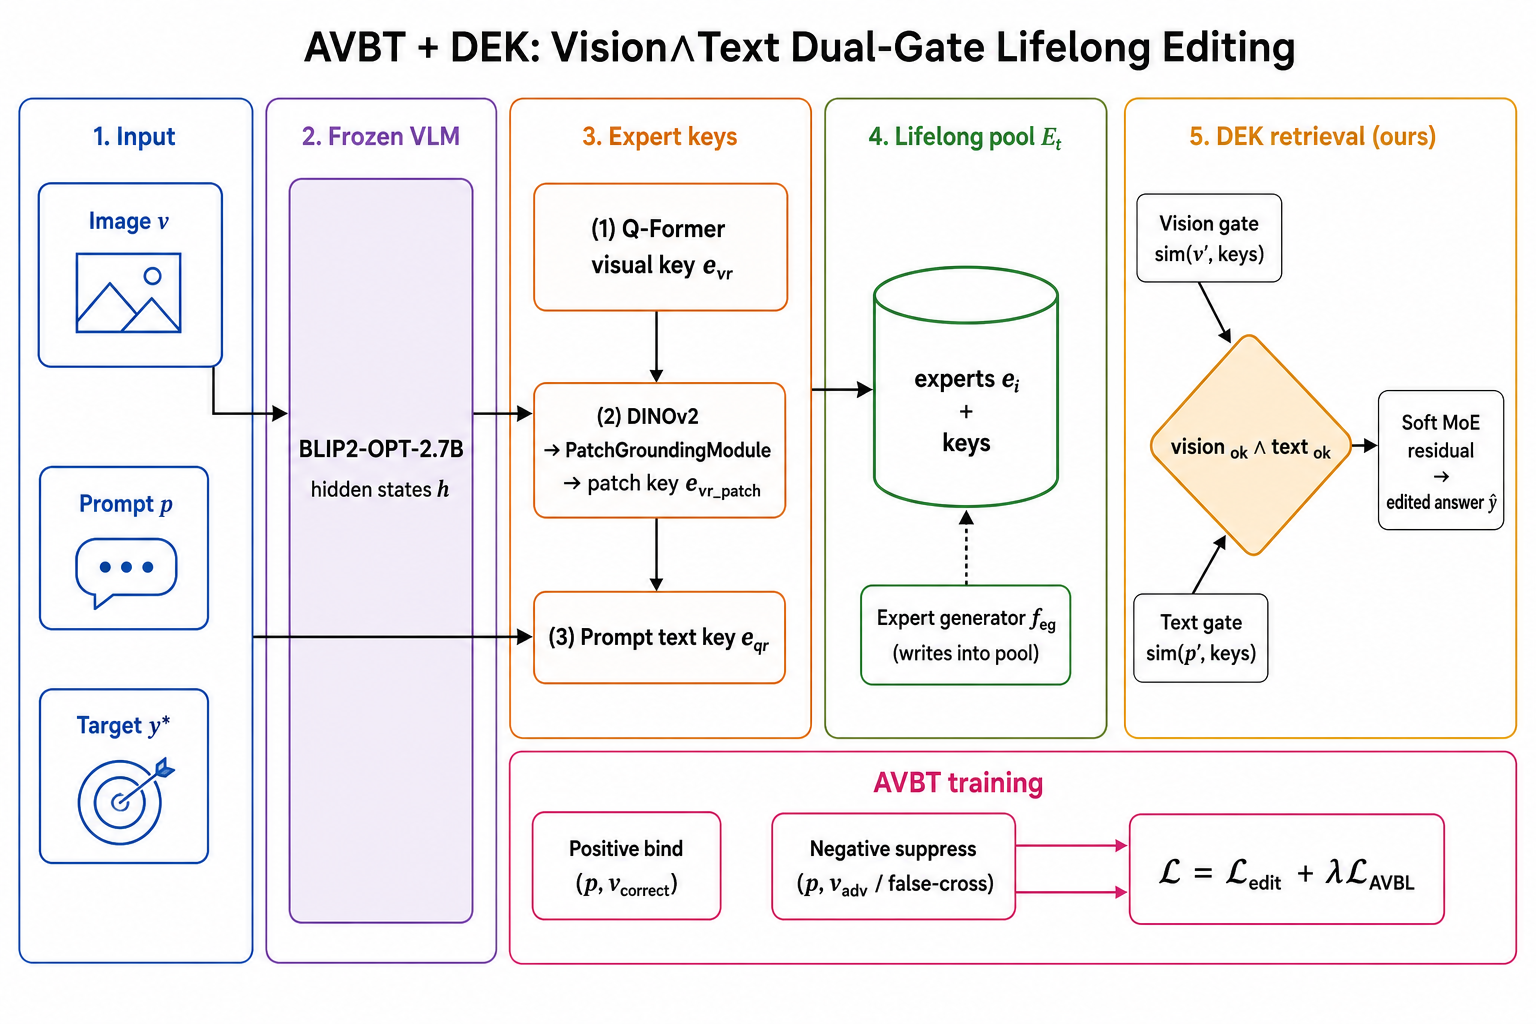
\includegraphics[width=0.72\textwidth,height=0.25\textheight,keepaspectratio]{Figures/architecture_avbt_dek.png}
\caption{Overview of AVBT + Dual-Expert Keys on a frozen VLM.
Each edit writes an MoE expert and separate vision/text keys into a lifelong pool.
AVBT trains positive binding on the edited image and suppression on adversarial images.
DEK retrieves only experts that pass both a vision gate and a text gate before soft MoE injection.}
\label{fig:arch}
\end{figure*}

\subsection{Expert pool and keys}
Let the frozen VLM be $f_\theta$.
An edit $(p_i,x_i,y_i)$ produces mid-layer representations from which we build:
(i)~an expert $e_i$ (low-rank MoE residual parameters);
(ii)~a Q-Former visual key $\mathbf{k}^{\mathrm{v}}_i$;
(iii)~a patch-grounded visual key $\mathbf{k}^{\mathrm{p}}_i$ from a DINOv2 patch grid passed through a small PatchGroundingModule;
(iv)~a prompt key $\mathbf{k}^{\mathrm{t}}_i$.
After $t$ edits the pool is
\begin{equation}
\mathcal{E}_t=\bigl\{\bigl(e_i,\mathbf{k}^{\mathrm{v}}_i,\mathbf{k}^{\mathrm{p}}_i,\mathbf{k}^{\mathrm{t}}_i\bigr)\bigr\}_{i=1}^{t}.
\label{eq:pool}
\end{equation}
On a query $(p',x')$ we extract query keys $(\mathbf{q}^{\mathrm{v}},\mathbf{q}^{\mathrm{p}},\mathbf{q}^{\mathrm{t}})$ in the same spaces.
Throughout, $\mathrm{sim}(\mathbf{u},\mathbf{v})$ denotes scaled cosine similarity between $\ell_2$-normalized vectors (equivalently a temperature-scaled dot product); the learned scale is absorbed into $\mathrm{sim}$ and is shared across vision and text routing.
Vision logits mix the Q-Former and patch scores (with a fixed fuse weight $\alpha\!\in\![0,1]$ when both are present):
\begin{equation}
s^{\mathrm{v}}_i
=
\alpha\,\mathrm{sim}\!\bigl(\mathbf{q}^{\mathrm{v}},\mathbf{k}^{\mathrm{v}}_i\bigr)
+
(1-\alpha)\,\mathrm{sim}\!\bigl(\mathbf{q}^{\mathrm{p}},\mathbf{k}^{\mathrm{p}}_i\bigr),
\label{eq:vis-logit}
\end{equation}
and likewise a text logit $s^{\mathrm{t}}_i=\mathrm{sim}(\mathbf{q}^{\mathrm{t}},\mathbf{k}^{\mathrm{t}}_i)$.
A non-edit ``prototype'' vision score $s^{\mathrm{v}}_{\mathrm{prot}}$ is computed from the query itself and acts as the no-edit baseline for the vision gate.


\subsection{Dual-Expert Keys}
False-positive retrieval is, in our logs, mostly a \emph{retrieval agreement} failure: a foreign expert clears a vision-only bar because its visual key collides with the query image.
DEK therefore stores vision and text keys separately and requires both modalities to agree before an expert may fire. 

% (Figure~\ref{fig:dek}).

A candidate $i$ first passes the vision gate if it beats the prototype,
\begin{equation}
\mathrm{vision\_ok}_i
\;=\;
\mathbb{I}\!\left[s^{\mathrm{v}}_i > s^{\mathrm{v}}_{\mathrm{prot}}\right].
\label{eq:vision-gate}
\end{equation}
Among the current pool we also score prompt-key agreement.
With margin $m\!\ge\!0$ (often $m{=}0$ in our runs), the text gate keeps only experts near the best text match:
\begin{equation}
\mathrm{text\_ok}_i
\;=\;
\mathbb{I}\!\left[s^{\mathrm{t}}_i \ge \max_{j}\,s^{\mathrm{t}}_j - m\right].
\label{eq:text-gate}
\end{equation}
Dual-Expert Keys retain expert $i$ only under the conjunction
\begin{equation}
r_i
\;=\;
\mathrm{vision\_ok}_i \;\wedge\; \mathrm{text\_ok}_i.
\label{eq:dek}
\end{equation}
Survivors are softly fused (softmax over gated vision logits) into a residual that is added at a chosen LLM layer; non-survivors contribute nothing.
The dual-gate is inference-time hygiene: it does not rewrite $f_\theta$, and it does not require the answer string to match $y_i$ before rejecting a foreign expert.
That is why FPR can fall sharply even when token-level image-swap remains only moderately improved.

% \begin{figure}[t]
% \centering
% \includegraphics[width=0.98\columnwidth]{Figures/fig_dek_dual_gate_v2.png}
% \caption{Dual-Expert Keys at retrieval.
% An expert survives only if it clears the vision gate against the no-edit prototype \emph{and} agrees with the prompt-key ranking (vision $\wedge$ text).}
% \label{fig:dek}
% \end{figure}

\subsection{Adversarial visual binding training}
Dual-Expert Keys (DEK) assume that keys are at least somewhat grounded.
Adversarial visual binding (AVBT) is the training counterpart: for each edit we optimize ordinary edit losses on the correct image, and we add an adversarial binding term on swap and hard-negative images built from the same prompt.

Let $\pi(\cdot)$ be the softmax routing distribution over pool experts plus the prototype slot, evaluated with binding-time vision scores.
On the correct image $x_i$, with own-expert index set $\mathcal{O}_i$, the positive term encourages mass on the true expert(s):
\begin{equation}
\mathcal{L}_{\mathrm{pos}}
=
-\log\!\left(\sum_{i\in\mathcal{O}_i}\pi_i(p_i,x_i)\right).
\label{eq:avbt-pos}
\end{equation}
On an adversarial image $x^{\mathrm{adv}}$ (swap or hard-negative) let $\pi^{\mathrm{adv}}$ be the same distribution, $m_{\mathrm{exp}}=\sum_{i\neq\mathrm{prot}}\pi^{\mathrm{adv}}_i$ the total expert mass, and $\pi^{\mathrm{adv}}_{\mathrm{prot}}$ the prototype probability.
With hinge threshold $\tau\!\ge\!0$ we penalize confident expert activation and push mass toward ``no edit'':
\begin{equation}
\mathcal{L}_{\mathrm{neg}}
=
\mathrm{ReLU}\!\left(m_{\mathrm{exp}}-\tau\right)\,
\bigl(-\log\pi^{\mathrm{adv}}_{\mathrm{prot}}\bigr)
+
\mathcal{L}_{\mathrm{aux}},
\label{eq:avbt-neg}
\end{equation}
where $\mathcal{L}_{\mathrm{aux}}$ collects light auxiliaries used in our runs (a margin on the top wrong expert and an optional contrastive push).
The adversarial visual binding objective is
\begin{equation}
\mathcal{L}_{\mathrm{bind}}
=
\mathcal{L}_{\mathrm{pos}}
+
\beta\,\mathcal{L}_{\mathrm{neg}},
\label{eq:avbt}
\end{equation}
and the full training loss is $\mathcal{L}=\mathcal{L}_{\mathrm{edit}}+\lambda\mathcal{L}_{\mathrm{bind}}$.
Unless noted otherwise we use $\lambda{=}0.3$, $\beta{=}2.5$, and $\tau{=}0.3$ with the contrastive auxiliary on.
Binding training alone does \emph{not} solve FPR on VLKEB (still $\approx\!96\%$): it reshapes attachment, but a vision-heavy retriever can still admit foreign experts.
That is why we treat Dual-Expert Keys as the primary anti-leakage mechanism and adversarial visual binding as supporting training.


% \subsection{What we do not promote as the method}
% We also tried false-cross neighbor mining and a larger pool buffer on top of DEK.
% They are reported as negative / secondary ablations neither unlocked a new image-swap regime, and the pool buffer worsened FPR.
% The method row we defend is AVBT training plus Dual-Expert Keys at retrieval.

\section{Experiments}
\label{sec:experiments}

We want the evaluation to answer one question cleanly: under adversarial images, does Dual-Expert Keys reduce false-positive retrieval without giving up reliability on the edited photograph?
Everything below is organized around that question rather than around chasing the highest token-swap score.

% \subsection{Backbone and editor testbed.}
\paragraph{Backbone and editor testbed.}
All primary runs use BLIP-2 OPT-2.7B as a frozen vision-language backbone~\cite{li2023blip2}.
We edit it with a LiveEdit-style lifelong MoE editor~\cite{chen2025liveedit}: each training edit writes a low-rank residual expert into a growing pool, and inference retrieves which expert(s) to inject.
We keep this architecture as the experimental testbed because continuous expert pools make wrong-expert retrieval observable; the scientific claim is about anti-leakage routing, not about beating LiveEdit on the original Rel, Gen or Loc leaderboard.
Weight-updating multimodal editors (Fine-tuning, MEND-VL, SERAC-VL)~\cite{Mitchell2021FastME,mitchell2022serac,cheng2023mmedit} appear as external comparisons.
They can change answers, but they do not expose a growing expert identity that we can score for FPR, so FPR is reported only for pool-based systems.
\begin{table*}[!ht]
\centering
\small
\setlength{\tabcolsep}{6pt}
\begin{tabular}{lcccccc}
\toprule
Method & Rel$\uparrow$ & T-Gen$\uparrow$ & M-Gen$\uparrow$ & T-Loc$\uparrow$ & M-Loc$\uparrow$ & FPR$\downarrow$ \\
\midrule
Lifelong baseline & 93.5 & 94.3 & 92.1 & 100 & 100 & 96 \\
Binding only & 93.8 & 94.5 & 93.8 & 100 & 100 & 96 \\
Dual-Expert Keys (ours) & 93.7 & 94.5 & 92.0 & 100 & 100 & \textbf{46} \\
\bottomrule
\end{tabular}
\caption{Main VLKEB result.
Standard metrics stay on parity with the lifelong baseline; Dual-Expert Keys cut false-positive retrieval $96\%\!\rightarrow\!46\%$.}
\label{tab:standard-vlkeb}
\end{table*}
% \subsection{Datasets and probes}
\paragraph{Datasets and probes.}
\label{sec:data-prep}
Our main benchmark is the original VLKEB multimodal editing dataset~\cite{huang2024vlkeb}.
Each VLKEB example already provides an edit triple $(p_i,x_i,y_i)$ together with the standard controls used in prior work: a text rephrase of $p_i$, an image rephrase of $x_i$, and text, multimodal locality items.
We keep those fields unchanged.
What VLKEB does not provide is an explicit test of whether retrieval still fires the right expert when the prompt is fixed and the image is wrong.
We therefore build an adversarial evaluation overlay on top of the original VLKEB splits rather than introducing a separate benchmark.

\paragraph{Construction.}
Starting from the original VLKEB train and eval JSONs and the VLKEB image root, we attach two extra image probes to every retained edit:
\begin{itemize}
\item \textbf{Image-swap:} Keep prompt $p_i$ and target $y_i$, but replace the image with $x_j$ from another VLKEB edit $j\neq i$.
Partners must come from a different entity folder in VLKEB's image layout, so the swapped photograph depicts a different scene or entity rather than a trivial crop of the same one.
\item \textbf{Hard-negative:} Keep $p_i$ and $y_i$, but replace the image with a confusable distractor that is also drawn from a different entity.
We prefer partners whose prompts share a coarse question skeleton with $p_i$ (same leading tokens), which makes the distractor harder than a random unrelated photograph.
\end{itemize}
If a candidate image file is missing on disk we skip that partner and try the next-ranked one; edits without a valid swap and hard-negative pair are dropped.
The resulting files still look like VLKEB rows: they retain Rel , Gen and Loc fields and simply add the two adversarial image paths used at evaluation (and, for binding training, at training).
Reliability, generality, and locality are therefore measured on the same VLKEB content as usual; only the adversarial probes are ours.

\paragraph{Training vs.\ evaluation use.}
The lifelong baseline is trained on the original VLKEB training edits.
Adversarial visual binding and Dual-Expert Keys additionally consume the adversarial images from the probe-augmented training split, because the binding loss needs swap , hard-negative views of each edit.
All primary tables evaluate the same probe-augmented VLKEB evaluation split under a frozen editor pool.
As a cross-dataset check we apply the identical pairing procedure to EasyEdit EVQA examples~\cite{wang2024easyedit}, again without changing the editor itself.

The probe suite used throughout is therefore:
(i)~reliability on the edited image $x_i$;
(ii)~image-swap;
(iii)~hard-negative;
(iv)~VLKEB text , image rephrase generality and locality~\cite{huang2024vlkeb,chen2025liveedit}.

% \subsection{Metrics}
\paragraph{Metrics.}
Standard multimodal editing metrics remain in the tables for context: reliability (Rel), text generality (T-Gen), multimodal generality (M-Gen), and text , multimodal locality (T-Loc , M-Loc)~\cite{cheng2023mmedit,huang2024vlkeb}.
On adversarial probes we also report answer-level image-swap and hard-negative accuracy, plus the reliability-swap gap.
Our primary novelty metric is \textbf{false-positive retrieval} (FPR): the fraction of adversarial queries for which routing activates at least one expert other than the intended edit (lower is better).
FPR is computed from routing logs under the same evaluation harness as Rel, swap; it is deliberately a retrieval-safety number, not a substitute for token accuracy.
When tables include both answer-level and routing metrics, we read them in that order: FPR first for the leakage claim, then Rel to confirm the edit still works, then swap, hard-negative and gap as secondary behaviour.

% \subsection{Baselines, comparisons, and ablations.}
\paragraph{Baselines, comparisons, and ablations}
We compare five rows that isolate mechanism:
\begin{itemize}
\item \textbf{Lifelong baseline:} LiveEdit-style MoE retrieval without adversarial visual binding and without Dual-Expert Keys.
\item \textbf{Binding only:} adversarial visual binding training with patch grounding, still using the original retrieval rule.
\item \textbf{Dual-Expert Keys (ours):} adversarial visual binding plus the vision~$\wedge$~text retrieval gate.
\item \textbf{Neighbor mining , pool buffer:} Dual-Expert Keys plus false-cross neighbor mining, or Dual-Expert Keys plus a larger pool buffer reported only as negative and secondary ablations.
\item \textbf{Fine-tuning, MEND-VL and SERAC-VL:} weight-updating multimodal editors under the same VLKEB probes.
\end{itemize}
In primary runs adversarial visual binding uses $\lambda{=}0.3$, $\beta{=}2.5$, hinge $\tau{=}0.3$, and the contrastive auxiliary described above.
Dual-Expert Keys applies the vision~$\wedge$~text conjunction gate; the text margin $m$ is held fixed across primary runs.


% \subsection{Evaluation protocol}
\paragraph{Evaluation protocol}
For the main VLKEB tables we evaluate $100$ edits with $10$ generations per example.
The headline ablation and competitor numbers use seed~$42$; multi-seed credibility uses five evaluation seeds $\{42,0,1,2,3\}$ on the same checkpoints.
EVQA stress follows the same three-way contrast lifelong baseline, binding only, and Dual-Expert Keys with a larger multi-seed subsample of $300$ edits when we report aggregate means and standard deviations.
Throughout, we log routing identities whenever false-positive retrieval is claimed.
We do \emph{not} treat token-level image-swap as a submission gate: the intended claim is a reduction in false-positive retrieval with reliability held.


\section{Results}
\label{sec:results}



Unless noted otherwise, all VLKEB numbers use the probe-augmented original evaluation split ($100$ edits, $10$ generations per example).
We lead with false-positive retrieval (FPR; lower is better) at reliability parity: that is the claim Dual-Expert Keys are designed to win.
Token-level image-swap is reported as secondary behaviour, not as a submission gate.

% \subsection{Main VLKEB result: FPR halves at Rel/Gen/Loc parity}
\subsection{False-positive retrieval on VLKEB}
Table~\ref{tab:standard-vlkeb} is the headline operating point.
Dual-Expert Keys preserve LiveEdit-style reliability, text,image generality, and locality, while cutting FPR from $96\%$ to $46\%$ a $50$~percentage-point absolute reduction.
Binding training alone leaves FPR unchanged at $96\%$: it can move answer scores on adversarial images, but it does not fix wrong-expert retrieval.
The dual vision-text gate is what changes the retrieval decision.



\subsection{What each component contributes}
% Figure~\ref{fig:results-ablation} and 

Table~\ref{tab:ablation} isolate the stack.
Moving from the lifelong baseline to binding-only training raises image-swap accuracy ($40.7\%\!\rightarrow\!47.8\%$) but leaves FPR at $96\%$.
Adding Dual-Expert Keys then collapses FPR to $46\%$ while reliability stays near $94\%$ and swap stays near the binding-only level.
Extra neighbor mining trims FPR only slightly ($46\%\!\rightarrow\!43\%$) without a swap gain; enlarging the pool buffer \emph{raises} FPR again to $55\%$.
We therefore treat neighbor mining and the pool buffer as negative ablations, not as part of the method row.

% \begin{figure}[!ht]
% \centering
% 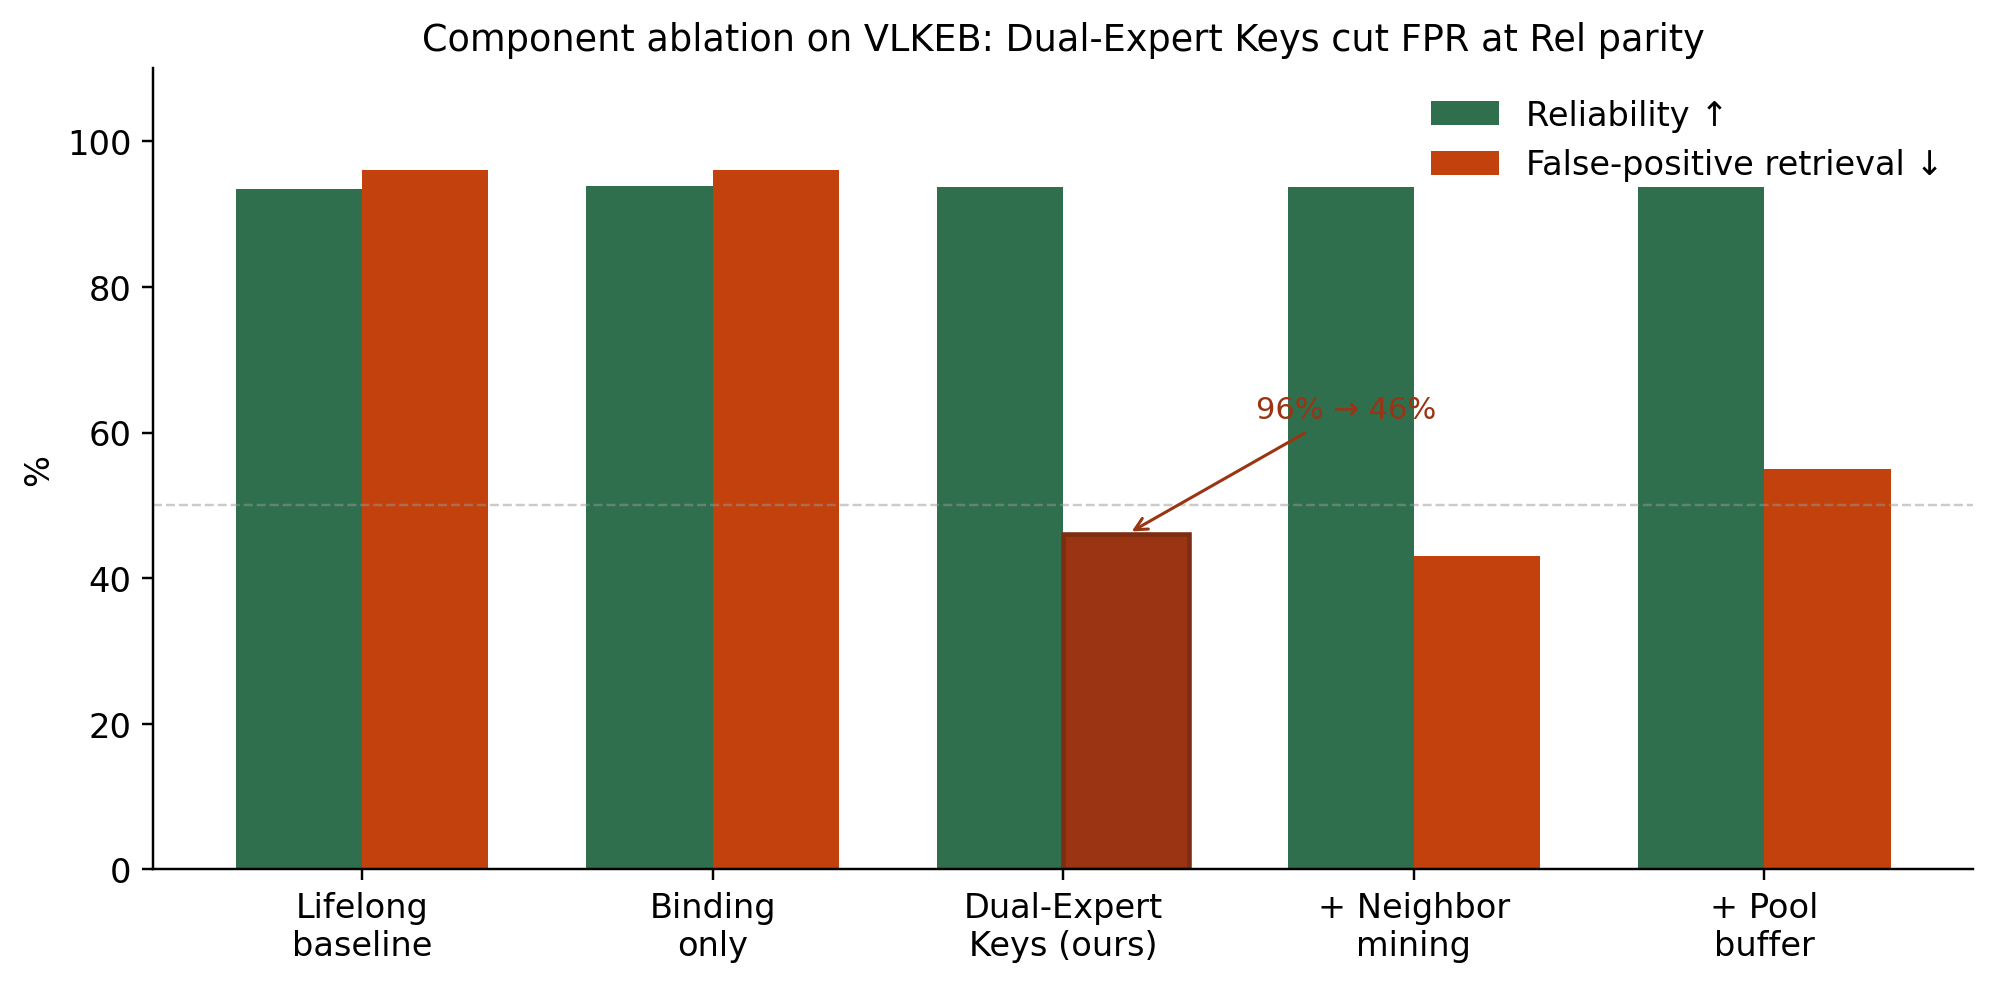
\includegraphics[width=\linewidth,height=0.22\textheight,keepaspectratio]{Figures/fig_results_ablation.png}
% \caption{Component ablation on VLKEB.
% Reliability stays high across rows; false-positive retrieval drops only when Dual-Expert Keys are added ($96\%\!\rightarrow\!46\%$).}
% \label{fig:results-ablation}
% \end{figure}

\begin{center}
\small
\setlength{\tabcolsep}{3pt}
\begin{tabular}{@{}lcccc@{}}
\toprule
Method & Rel$\uparrow$ & Swap$\uparrow$ & FPR$\downarrow$ & Role \\
\midrule
Lifelong baseline & 93.5 & 40.7 & 96 & baseline \\
Binding only & 93.8 & 47.8 & 96 & +binding \\
Dual-Expert Keys & 93.7 & 47.7 & \textbf{46} & +dual gate \\
+ Neighbor mining & 93.7 & 47.2 & 43 & negative \\
+ Pool buffer & 93.7 & 48.0 & 55 & negative \\
\bottomrule
\end{tabular}
\captionof{table}{Ablation of the lifelong editor family on VLKEB (seed~$42$).
Dual-Expert Keys are the FPR mechanism; binding alone is not.}
\label{tab:ablation}
\end{center}

\subsection{Multi-seed stability and significance}
Figure~\ref{fig:results-multiseed} and Table~\ref{tab:multiseed} repeat the lifelong-baseline vs.\ Dual-Expert Keys comparison over five evaluation seeds on the same checkpoints.
FPR is $96\%$ for the baseline and $46\%$ for Dual-Expert Keys on \emph{every} seed ($-50$~pp, no regression).
Mean image-swap rises from $41.2\%$ to $48.6\%$ ($+7.4$~pp; paired $t$-test, $n{=}5$, two-sided $p{=}3.4{\times}10^{-4}$).
Reliability remains held ($93.5\%$ vs.\ $93.7\%$).
The FPR win is therefore not a single-seed artefact: the dual-gate decides retrieval in a stable way, and the modest swap lift is statistically significant.

\begin{figure}[!ht]
\centering
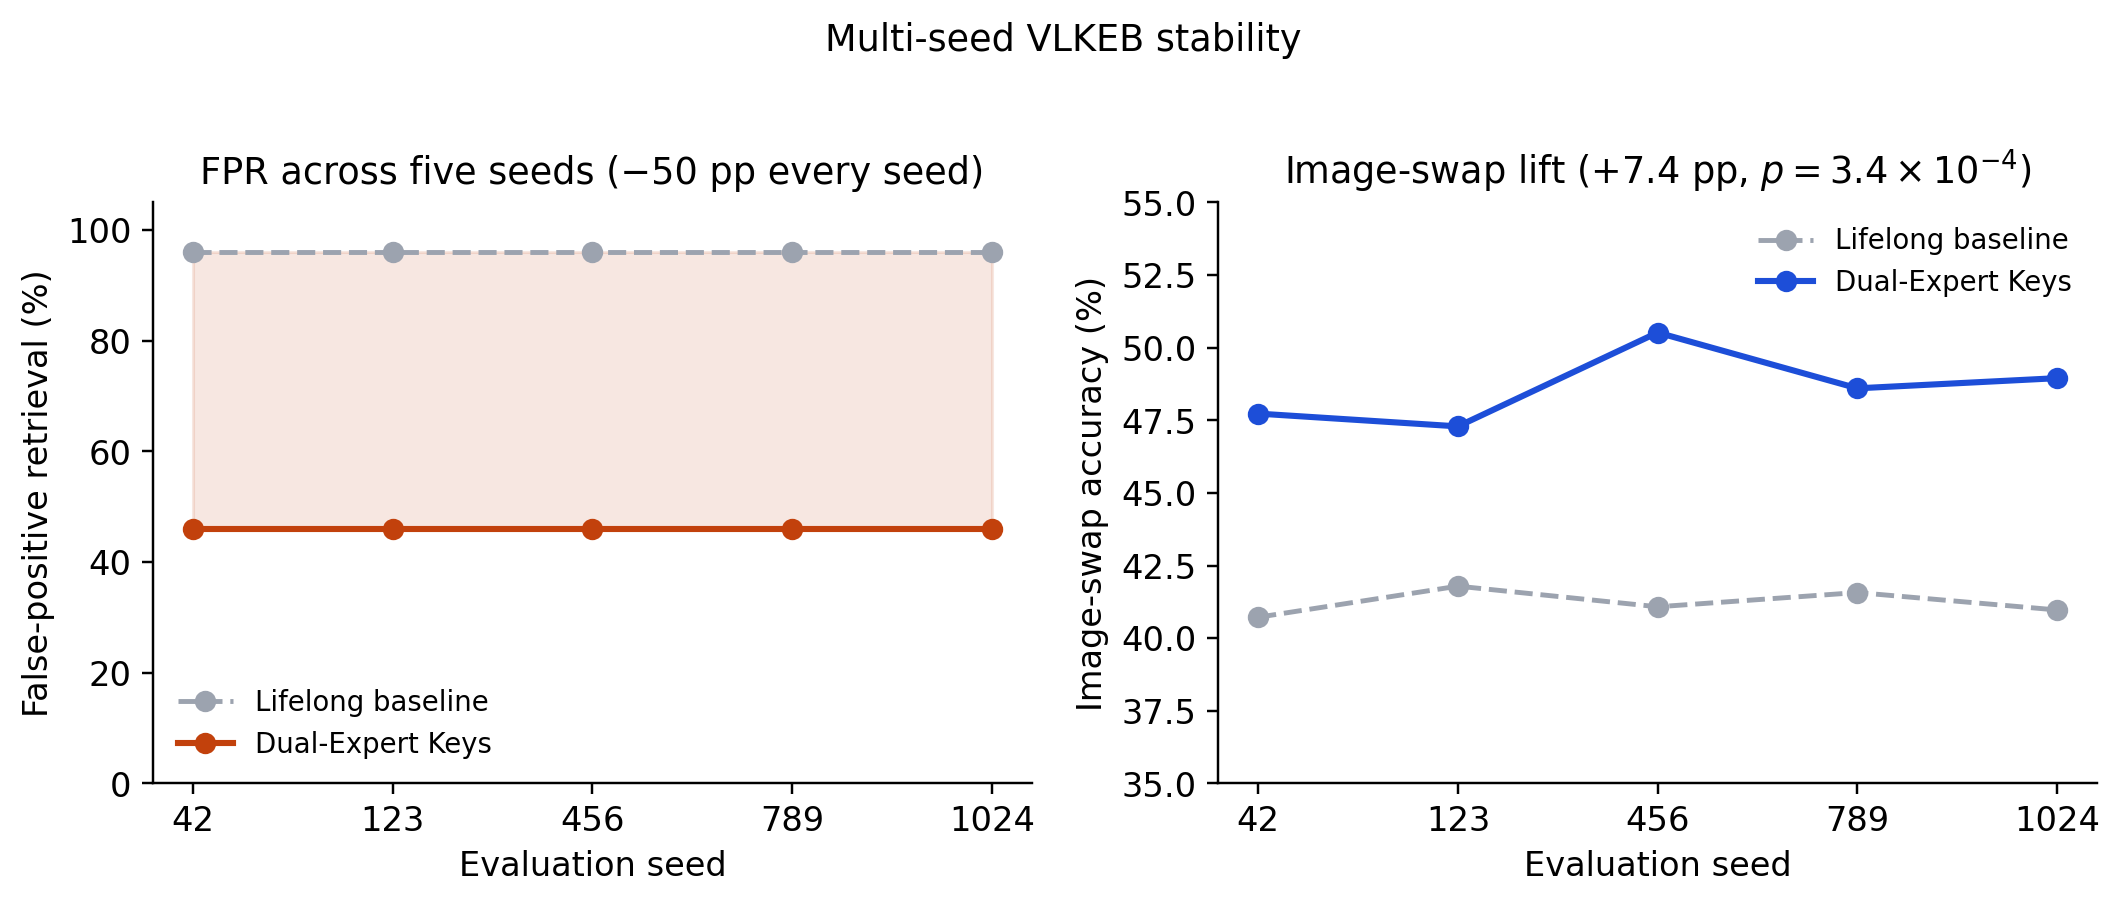
\includegraphics[width=\linewidth,height=0.20\textheight,keepaspectratio]{Figures/fig_results_multiseed.png}
\caption{Five-seed VLKEB stability.
Left: false-positive retrieval stays at $46\%$ for Dual-Expert Keys versus $96\%$ for the lifelong baseline on every seed.
Right: image-swap accuracy improves on every seed ($+7.4$~pp mean).}
\label{fig:results-multiseed}
\end{figure}

\begin{center}
\small
\begin{tabular}{@{}lcccc@{}}
\toprule
Method & Rel$\uparrow$ & Swap$\uparrow$ & FPR$\downarrow$ & Swap-gap$\downarrow$ \\
\midrule
Lifelong baseline & $93.5$ & $41.2{\pm}0.4$ & $96.0$ & $52.2{\pm}0.4$ \\
Dual-Expert Keys & $93.7$ & $\mathbf{48.6{\pm}1.3}$ & $\mathbf{46.0}$ & $45.1{\pm}1.3$ \\
\bottomrule
\end{tabular}
\captionof{table}{Multi-seed VLKEB summary (mean $\pm$ std over five seeds; Rel/FPR constant across seeds here).
Swap lift $+7.4$~pp ($p{=}3.4{\times}10^{-4}$); FPR $-50$~pp.}
\label{tab:multiseed}
\end{center}

\subsection{Comparison to weight-updating editors}
% Figure~\ref{fig:results-competitors} and 

Table~\ref{tab:competitors} place Dual-Expert Keys next to Fine-tuning, MEND-VL, and SERAC-VL under the same VLKEB probes.
The external editors either under-edit or collapse reliability: Fine-tuning and MEND-VL sit near $71$-$73\%$ Rel with almost no reliability-swap gap, and SERAC-VL falls to $\approx\!39\%$ Rel.
None of them expose a growing expert identity, so FPR is not defined for those rows.
Among systems that \emph{do} maintain a lifelong pool, Dual-Expert Keys are the only setting that keeps Rel near $94\%$ while cutting FPR in half.
That is the intended contrast: not a race for the highest adversarial token score, but a high-reliability anti-leakage operating point.

% \begin{figure}[!ht]
% \centering
% 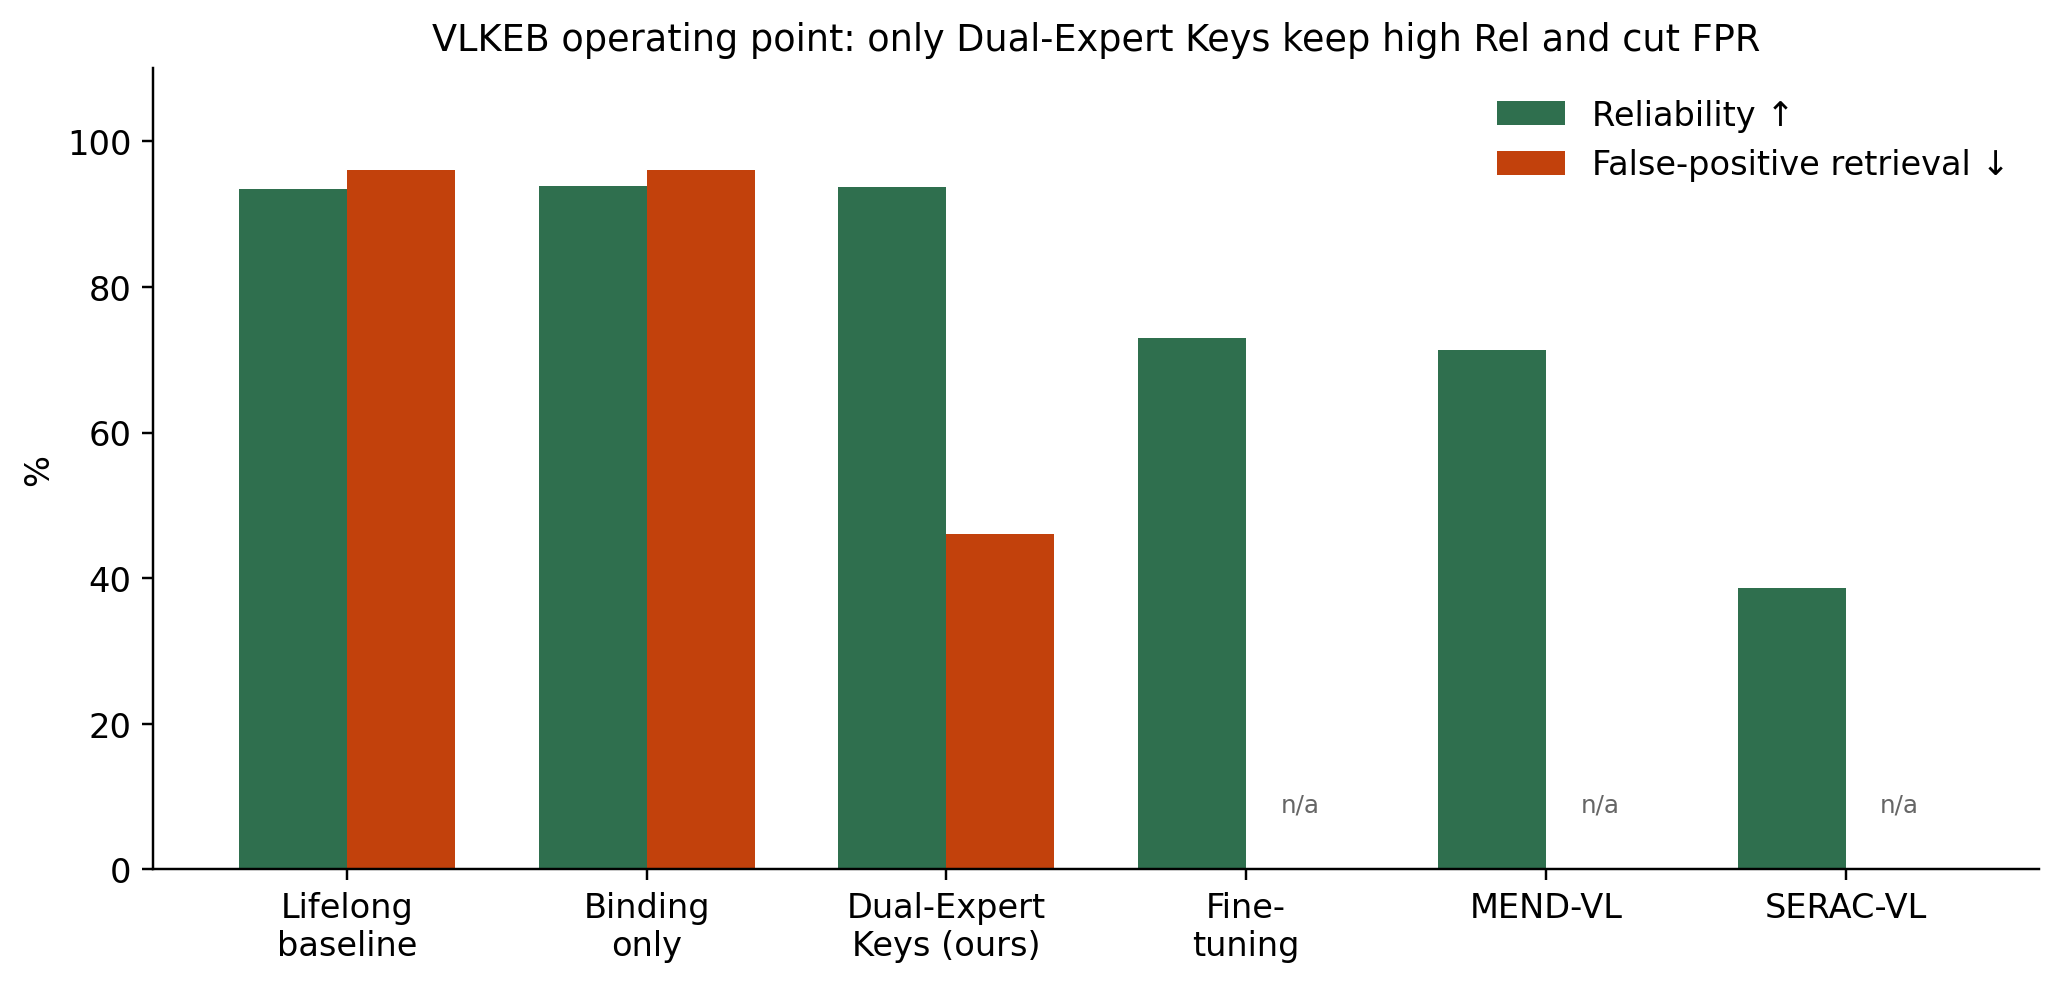
\includegraphics[width=\linewidth,height=0.20\textheight,keepaspectratio]{Figures/fig_results_competitors.png}
% \caption{VLKEB operating-point comparison.
% Dual-Expert Keys uniquely combine high reliability with a large FPR cut; Fine-tuning / MEND-VL / SERAC-VL lack a pool FPR score.}
% \label{fig:results-competitors}
% \end{figure}

\begin{center}
\small
\setlength{\tabcolsep}{3pt}
\begin{tabular}{@{}lcccc@{}}
\toprule
Method & Rel$\uparrow$ & Swap$\uparrow$ & Swap-gap$\downarrow$ & FPR$\downarrow$ \\
\midrule
Lifelong baseline & 93.5 & 40.7 & 52.8 & 96 \\
Binding only & 93.8 & 47.8 & 46.0 & 96 \\
Dual-Expert Keys (ours) & 93.7 & 47.7 & 46.0 & \textbf{46} \\
Fine-tuning & 73.0 & 73.1 & $\approx$0 & n/a \\
MEND-VL & 71.3 & 69.4 & 1.9 & n/a \\
SERAC-VL & 38.6 & 38.6 & $\approx$0 & n/a \\
\bottomrule
\end{tabular}
\captionof{table}{Competitors on VLKEB probes (seed~$42$).
FPR applies only to retrieval-pool editors.}
\label{tab:competitors}
\end{center}

\subsection{Cross-dataset stress on EVQA}
To check that the FPR story is not VLKEB-specific, we apply the same probe construction and the same lifelong-baseline , binding-only and Dual-Expert Keys contrast to EasyEdit EVQA~\cite{wang2024easyedit}.
% Figure~\ref{fig:results-evqa} and 
Table~\ref{tab:evqa} summarize five evaluation seeds with $300$ edits each.
Reliability stays near $95\%$ for all three rows.
Binding only again tracks the lifelong baseline on FPR.
Dual-Expert Keys reduce image-swap FPR to $1.5\%{\pm}1.1\%$ and hard-negative FPR to $2.7\%{\pm}1.3\%$ more than an order of magnitude below the baseline hard-negative leakage ($96.8\%{\pm}0.6\%$).
Token-level swap on EVQA remains low for every method; we do not claim an EVQA swap leaderboard.
The transferable message is the same as on VLKEB: Dual-Expert Keys suppress wrong-expert retrieval while holding reliability.

% \begin{figure}[!ht]
% \centering
% 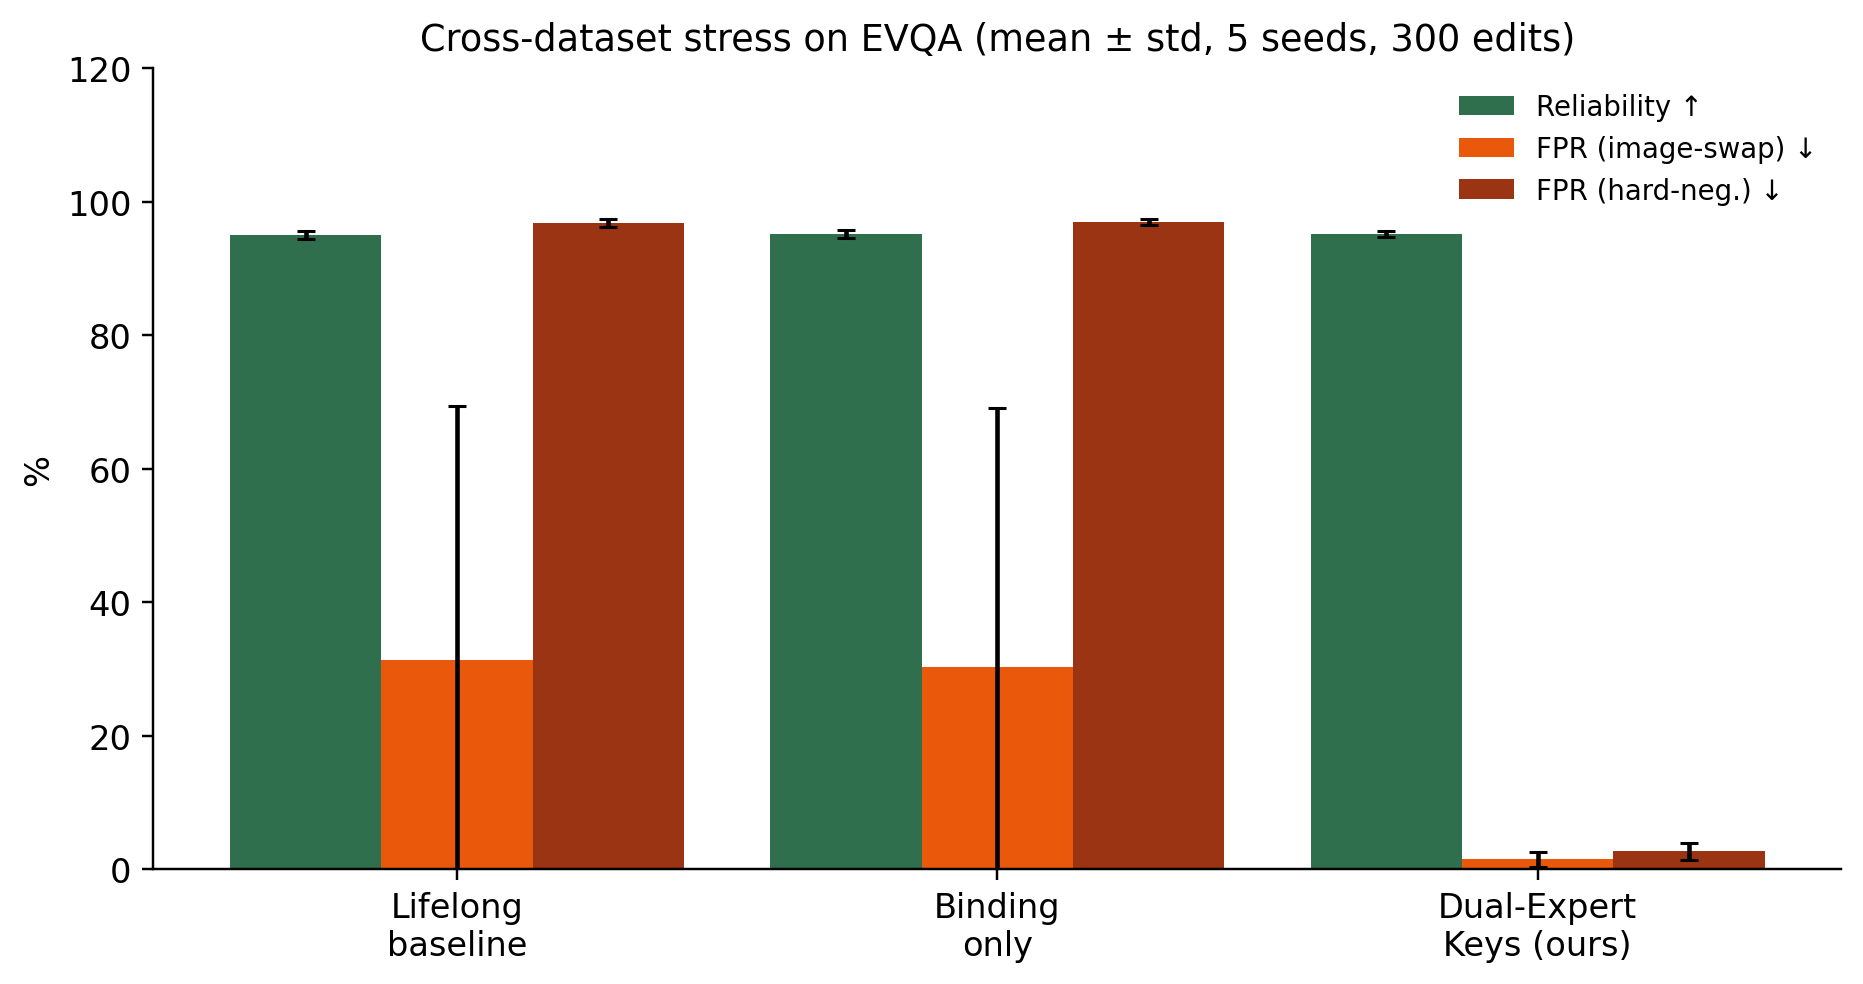
\includegraphics[width=\linewidth,height=0.20\textheight,keepaspectratio]{Figures/fig_results_evqa.png}
% \caption{EVQA cross-dataset stress (mean $\pm$ std over five seeds).
% Dual-Expert Keys collapse swap and hard-negative FPR while Rel stays near $95\%$.}
% \label{fig:results-evqa}
% \end{figure}

\begin{center}
\small
\begin{tabular}{@{}lccc@{}}
\toprule
Method & Rel$\uparrow$ & FPR$_{\mathrm{swap}}\downarrow$ & FPR$_{\mathrm{hard}}\downarrow$ \\
\midrule
Lifelong baseline & $95.0{\pm}0.6$ & $31.3{\pm}38.1$ & $96.8{\pm}0.6$ \\
Binding only & $95.2{\pm}0.6$ & $30.3{\pm}38.8$ & $97.0{\pm}0.4$ \\
Dual-Expert Keys & $\mathbf{95.2{\pm}0.5}$ & $\mathbf{1.5{\pm}1.1}$ & $\mathbf{2.7{\pm}1.3}$ \\
\bottomrule
\end{tabular}
\captionof{table}{EVQA multi-seed grounding stress ($300$ edits per seed).
Means $\pm$ std over seeds $\{42,0,1,2,3\}$.}
\label{tab:evqa}
\end{center}

% Taken together, the VLKEB main table, the ablation, the five-seed significance check, the competitor contrast, and the EVQA stress support one claim:
% \emph{Dual-Expert Keys deliver a large, stable reduction in false-positive retrieval with reliability held; adversarial visual binding is helpful supporting training, not a substitute for the dual gate.}
% \section{Limitations}
% The results above establish a clear win on the metric we set out to improve: Dual-Expert Keys cut false-positive retrieval while preserving high reliability.
% What follows only situates that win.

% Our primary success criterion is retrieval safety rather than adversarial token accuracy.
% Image-swap answer rates still leave headroom, which we treat as a separate, harder generation problem for the frozen decoder not as evidence that the dual gate failed.
% Stopping the wrong expert from firing is already a substantial gain even when the model does not always refuse the edited answer string on a mismatched photograph.

% False-positive retrieval is also scoped to lifelong editors with an identifiable expert pool, which is exactly where leakage is observable and actionable.
% Weight-updating editors such as Fine-tuning, MEND-VL, and SERAC-VL remain useful operating-point baselines, but they do not admit the same expert-identity score.
% Marking FPR as n/a for those rows is therefore a property of the metric, not a shortcoming of Dual-Expert Keys.

% Finally, the main evidence uses BLIP-2 OPT-2.7B on VLKEB, complemented by a completed EVQA cross-dataset stress that reproduces the same FPR pattern~\cite{li2023blip2,huang2024vlkeb,wang2024easyedit}.
% Together those settings cover both the primary editing benchmark and an out-of-distribution probe set under the same dual-gate rule.
\section{Limitations}
Our primary claim is retrieval safety, not token-level image-swap accuracy; residual swap answer headroom is a separate generation problem for the frozen decoder.
False-positive retrieval is also defined only for lifelong editors with an identifiable expert pool, so FPR is n/a for weight-updating baselines such as Fine-tuning, MEND-VL, and SERAC-VL.
The main evidence uses BLIP-2 OPT-2.7B on VLKEB, with EVQA as a completed cross-dataset check under the same dual-gate rule~\cite{li2023blip2,huang2024vlkeb,wang2024easyedit}.

\section{Conclusion}
Lifelong multimodal editors can look correct on the image they were edited for and still retrieve the wrong stored fact when the scene changes.
We identify that failure as \emph{false-positive retrieval} and show that standard metric scores do not catch it.
Dual-Expert Keys fix the decision rule: an expert may fire only when vision and text agree.
Adversarial visual binding strengthens edit-image attachment during training so the dual gate is not fighting weakly grounded keys.

% Empirically the combination works.
These mechanisms translate into large, stable reductions in false-positive retrieval.
On original VLKEB with our adversarial probes, Dual-Expert Keys reduce false-positive retrieval from $96\%$ to $46\%$ while keeping reliability near $94\%$.
The cut is stable across five evaluation seeds, survives comparison against Fine-tuning, MEND-VL, and SERAC-VL at a high-reliability operating point, and reappears under EVQA stress.
Binding training alone does not deliver the FPR win; the dual gate does.
Taken together, these results show that lifelong multimodal editing can be made substantially safer at retrieval time without sacrificing the reliability that existing benchmarks already reward.


\bibliography{aaai2027}

% Check whether the conference requires a reproducibility checklist to be included in the paper.
% If so, you can uncomment the following line and ajust the path to include it.
% \makeatletter
\@ifundefined{isChecklistMainFile}{
  % We are compiling a standalone document
  \newif\ifreproStandalone
  \reproStandalonetrue
}{
  % We are being \input into the main paper
  \newif\ifreproStandalone
  \reproStandalonefalse
}
\makeatother

\ifreproStandalone
\documentclass[letterpaper]{article}
\usepackage[submission]{aaai2027}
\setlength{\pdfpagewidth}{8.5in}
\setlength{\pdfpageheight}{11in}
\frenchspacing

\begin{document}
\fi
\setlength{\leftmargini}{20pt}
\makeatletter\def\@listi{\leftmargin\leftmargini \topsep .5em \parsep .5em \itemsep .5em}
\def\@listii{\leftmargin\leftmarginii \labelwidth\leftmarginii \advance\labelwidth-\labelsep \topsep .4em \parsep .4em \itemsep .4em}
\def\@listiii{\leftmargin\leftmarginiii \labelwidth\leftmarginiii \advance\labelwidth-\labelsep \topsep .4em \parsep .4em \itemsep .4em}\makeatother

\setcounter{secnumdepth}{0}
\renewcommand\thesubsection{\arabic{subsection}}
\renewcommand\labelenumi{\thesubsection.\arabic{enumi}}

\newcounter{checksubsection}
\newcounter{checkitem}[checksubsection]

\newcommand{\checksubsection}[1]{%
  \refstepcounter{checksubsection}%
  \paragraph{\arabic{checksubsection}. #1}%
  \setcounter{checkitem}{0}%
}

\newcommand{\checkitem}{%
  \refstepcounter{checkitem}%
  \item[\arabic{checksubsection}.\arabic{checkitem}.]%
}
\newcommand{\question}[2]{\normalcolor\checkitem #1 #2 \color{blue}}
\newcommand{\ifyespoints}[1]{\makebox[0pt][l]{\hspace{-15pt}\normalcolor #1}}

\section*{Reproducibility Checklist}

\vspace{1em}
\hrule
\vspace{1em}

\textbf{Instructions for Authors:}

This document outlines key aspects for assessing reproducibility. Please provide your input by editing this \texttt{.tex} file directly.

For each question (that applies), replace the ``Type your response here'' text with your answer.

\vspace{1em}
\noindent
\textbf{Example:} If a question appears as
%
\begin{center}
\noindent
\begin{minipage}{.9\linewidth}
\ttfamily\raggedright
\string\question \{Proofs of all novel claims are included\} \{(yes/partial/no)\} \\
Type your response here
\end{minipage}
\end{center}
you would change it to:
\begin{center}
\noindent
\begin{minipage}{.9\linewidth}
\ttfamily\raggedright
\string\question \{Proofs of all novel claims are included\} \{(yes/partial/no)\} \\
yes
\end{minipage}
\end{center}
%
Please make sure to:
\begin{itemize}\setlength{\itemsep}{.1em}
\item Replace ONLY the ``Type your response here'' text and nothing else.
\item Use one of the options listed for that question (e.g., \textbf{yes}, \textbf{no}, \textbf{partial}, or \textbf{NA}).
\item \textbf{Not} modify any other part of the \texttt{\string\question} command or any other lines in this document.\\
\end{itemize}

You can \texttt{\string\input} this .tex file right before \texttt{\string\end\{document\}} of your main file or compile it as a stand-alone document. Check the instructions on your conference's website to see if you will be asked to provide this checklist with your paper or separately.

\vspace{1em}
\hrule
\vspace{1em}

% The questions start here

\checksubsection{General Paper Structure}
\begin{itemize}

\question{Includes a conceptual outline and/or pseudocode description of AI methods introduced}{(yes/partial/no/NA)}
Type your response here

\question{Clearly delineates statements that are opinions, hypothesis, and speculation from objective facts and results}{(yes/no)}
Type your response here

\question{Provides well-marked pedagogical references for less-familiar readers to gain background necessary to replicate the paper}{(yes/no)}
Type your response here

\end{itemize}
\checksubsection{Theoretical Contributions}
\begin{itemize}

\question{Does this paper make theoretical contributions?}{(yes/no)}
Type your response here

	\ifyespoints{\vspace{1.2em}If yes, please address the following points:}
        \begin{itemize}
	
	\question{All assumptions and restrictions are stated clearly and formally}{(yes/partial/no)}
	Type your response here

	\question{All novel claims are stated formally (e.g., in theorem statements)}{(yes/partial/no)}
	Type your response here

	\question{Proofs of all novel claims are included}{(yes/partial/no)}
	Type your response here

	\question{Proof sketches or intuitions are given for complex and/or novel results}{(yes/partial/no)}
	Type your response here

	\question{Appropriate citations to theoretical tools used are given}{(yes/partial/no)}
	Type your response here

	\question{All theoretical claims are demonstrated empirically to hold}{(yes/partial/no/NA)}
	Type your response here

	\question{All experimental code used to eliminate or disprove claims is included}{(yes/no/NA)}
	Type your response here
	
	\end{itemize}
\end{itemize}

\checksubsection{Dataset Usage}
\begin{itemize}

\question{Does this paper rely on one or more datasets?}{(yes/no)}
Type your response here

\ifyespoints{If yes, please address the following points:}
\begin{itemize}

	\question{A motivation is given for why the experiments are conducted on the selected datasets}{(yes/partial/no/NA)}
	Type your response here

	\question{All novel datasets introduced in this paper are included in a data appendix}{(yes/partial/no/NA)}
	Type your response here

	\question{All novel datasets introduced in this paper will be made publicly available upon publication of the paper with a license that allows free usage for research purposes}{(yes/partial/no/NA)}
	Type your response here

	\question{All datasets drawn from the existing literature (potentially including authors' own previously published work) are accompanied by appropriate citations}{(yes/no/NA)}
	Type your response here

	\question{All datasets drawn from the existing literature (potentially including authors' own previously published work) are publicly available}{(yes/partial/no/NA)}
	Type your response here

	\question{All datasets that are not publicly available are described in detail, with explanation why publicly available alternatives are not scientifically satisficing}{(yes/partial/no/NA)}
	Type your response here

\end{itemize}
\end{itemize}

\checksubsection{Computational Experiments}
\begin{itemize}

\question{Does this paper include computational experiments?}{(yes/no)}
Type your response here

\ifyespoints{If yes, please address the following points:}
\begin{itemize}

	\question{This paper states the number and range of values tried per (hyper-) parameter during development of the paper, along with the criterion used for selecting the final parameter setting}{(yes/partial/no/NA)}
	Type your response here

	\question{Any code required for pre-processing data is included in the appendix}{(yes/partial/no)}
	Type your response here

	\question{All source code required for conducting and analyzing the experiments is included in a code appendix}{(yes/partial/no)}
	Type your response here

	\question{All source code required for conducting and analyzing the experiments will be made publicly available upon publication of the paper with a license that allows free usage for research purposes}{(yes/partial/no)}
	Type your response here
        
	\question{All source code implementing new methods have comments detailing the implementation, with references to the paper where each step comes from}{(yes/partial/no)}
	Type your response here

	\question{If an algorithm depends on randomness, then the method used for setting seeds is described in a way sufficient to allow replication of results}{(yes/partial/no/NA)}
	Type your response here

	\question{This paper specifies the computing infrastructure used for running experiments (hardware and software), including GPU/CPU models; amount of memory; operating system; names and versions of relevant software libraries and frameworks}{(yes/partial/no)}
	Type your response here

	\question{This paper formally describes evaluation metrics used and explains the motivation for choosing these metrics}{(yes/partial/no)}
	Type your response here

	\question{This paper states the number of algorithm runs used to compute each reported result}{(yes/no)}
	Type your response here

	\question{Analysis of experiments goes beyond single-dimensional summaries of performance (e.g., average; median) to include measures of variation, confidence, or other distributional information}{(yes/no)}
	Type your response here

	\question{The significance of any improvement or decrease in performance is judged using appropriate statistical tests (e.g., Wilcoxon signed-rank)}{(yes/partial/no)}
	Type your response here

	\question{This paper lists all final (hyper-)parameters used for each model/algorithm in the paper’s experiments}{(yes/partial/no/NA)}
	Type your response here


\end{itemize}
\end{itemize}
\ifreproStandalone
\end{document}
\fi


\end{document}
